\graphicspath{{chapters/loadings/}}
\chapter{Regularization and the Interpretation of \acrshort{cca} Weights and Loadings}\label{chap:loadings}
\minitoc
% chktex-file 44
% chktex-file 3
\epigraph{If you change the way you look at things, the things you look at change.}{\textit{Wayne Dyer}}
\epigraph{He was constantly reminded of how startlingly different a place the world was when viewed from a point only three feet to the left.}{\textit{Douglas Adams}}
\section{Introduction}

The application of Canonical Correlation Analysis (\acrshort{cca}) methods to practical problems often involves two key aspects: predicting latent variables associated with different views, and understanding the nature of the relationship between these views.
This dichotomy in goals bears resemblance to the distinction between machine learning and probabilistic or statistical approaches to the \acrshort{cca} problem.
Machine learning approaches prioritize (out-of-sample) prediction of latent variables for downstream tasks, while statistical approaches seek to infer the data generation process from latent variables to the observed data.
Notably, the probabilistic approach to \acrshort{cca} focusses on the forward model from latent variables to observed data, while the machine learning approach focusses on the inverse model from observed data to latent variables.
As a result the probabilistic \acrshort{cca} is parameterized by the \textit{loadings} (parameters that transform latent variables to observed data), while the machine learning approach is parameterized by \textit{weights} (parameters that transform obsevred data to latent variables).
We would ideally like to have the best possible prediction of the latent variables, while also being able to interpret the model and understand the relationship between the views.
This implies that we would like to have models which are both good at prediction and have interpretable \gls{loadings} that we can use to understand the relationship between the views via the data generation process.
The importance of the \gls{loadings} (associated with the `forward' model from latent variables to observed data) instead of weights (associated with the `backward' model from observed data to latent variables) for interpretability was highlighted by \cite{haufe2014interpretation} for linear models including \acrshort{svm} and Lasso, along with methods for transforming `backward' weights to `forward' loadings.
We contribute to this line of work by demonstrating a similar relationship between the \gls{loadings} and weights of \acrshort{cca} models, and showing that the \gls{loadings} are more interpretable than the weights.

In this chapter, we reexamine the relationship between machine learning and probabilistic \acrshort{cca} approaches using simulated data.
We demonstrate that these approaches are more aligned than previously thought.
While sparse regularization of \acrshort{cca} weights can lead to sparse estimates of generative model \gls{loadings} in some conditions, it doesn't always ensure sparse loadings, especially under anisotropic noise (i.e. noise correlated between features).

\section{Background:Generative Perspectives on \acrshort{cca}}

Understanding the data generation process in \acrshort{cca} and \acrshort{pls} is pivotal for many reasons.
It influences the choice of appropriate models, evaluation metrics, and sheds light on the underlying structure and dependencies between views.
Probabilistic formulations provide a principled framework to understand this process, helping us gauge the assumptions we make and the limitations these impose.

\subsection{Probabilistic \acrshort{cca} and \acrshort{gfa} (Explicit Latent Variable Models)}\label{subsubsec:a-probabilistic-latent-variable-perspective}


% #TODO: Weights are combinations of subsets of features in each view that covary/correlate
% #TODO: Loadings are correlations of each feature with the latent variable

Consider the graphical model depicted in Figure~\ref{fig:mentalhealthselfsupervised}.
It comprises two distinct views: a neuroimaging modality and a behavioral modality.
Both views are assumed to originate from a common latent variable, representing the severity of a mental health condition.
The neuroimaging modality is generated via a linear model with added noise, while the behavioral modality similarly arises from a linear model with noise.
Consequently, the brain and behavioral modalities exhibit correlation since they both derive from the same latent variable.
In a statistical sense, they are conditionally independent, given the latent variable.

\begin{figure}
    \centering
    \tikz{
        % nodes
        \node[latent, align=center, minimum size=2cm] (Z) {Severity\\z};
        %
        \node[obs, below left=of Z, minimum size=2cm, align=center] (x1) {Brain\\$x^{(1)}$};
        \node[obs, below right=of Z, minimum size=2cm, align=center] (x2) {Behaviour\\$x^{(2)}$};
        % edges
        \edge{Z} {x1}
        \edge{Z} {x2}}
    \caption[Latent Variable Model of Mental Health]{\textit{\textbf{Latent Variable Model of Mental Health:}} From this perspective the neuroimaging modality and behavioural data are both considered to have been generated with distributions conditioned on the severity of a mental health condition}\label{fig:mentalhealthselfsupervised}
\end{figure}

The distributions of the two views are given by:

\begin{align}
    z& \sim \mathcal{N}(0, I)\\
    x\sps{i} & \sim \mathcal{N}(W\sps{i} z + \mu\sps{i}, \Psi\sps{i})
\end{align}

Where \(z\) represents the latent variable (disease severity), \(x\sps{i}\) represents the $i^{\text{th}}$ view, \(W\sps{i}\) represents the model loadings, \(\mu\sps{i}\) represents the mean, and \(\Psi\sps{i}\) represents the noise covariance matrix for the $i^{\text{th}}$ view.
Notice that if it were not for the view-specific noise, the two views would be perfectly correlated subject to a linear transformation.

\citep{bach2005probabilistic} showed that the maximum likelihood solution for this model is equivalent to the solution of the \acrshort{cca} problem in the sense that the \gls{loadings} are the same as the \acrshort{cca} weights multiplied by the covariance:

\begin{align}\label{eq:probabilistic-cca}
    \hat{W}\sps{i} = \Sigma_{ii} \hat{U}\sps{i} R
\end{align}

Where $R$ is an arbitrary rotation matrix and $\hat{U}\sps{i}$ is the matrix of \acrshort{cca} weights for the $i$th view.
This implies that for invertible covariance matrices, we can access the `true' \acrshort{cca} weights by multiplying the \gls{loadings} by the inverse of the covariance matrix:

\begin{align}
    \hat{U}\sps{i} = \Sigma_{ii}^{-1} \hat{W}\sps{i}
\end{align}

In practice we do not have access to the covariance matrices $\Sigma_{ii}$, so we must estimate them from the data using the sample covariance matrices $\hat{\Sigma}_{ii}$.

Notice that for Identity covariance matrices, the \acrshort{cca} weights are the same as the loadings.
Otherwise, there is a linear transformation between the two.
For singular covariance matrices, the \acrshort{cca} weights are not uniquely defined.

Moreover, the mean of the posterior distribution of the latent variables is proportional to the mean of the \acrshort{cca} scores\citep{klami2013bayesian}.
Group Factor Analysis (\acrshort{gfa}) is a closely related model that assumes diagonal covariance in $\Psi\sps{i}$:

\begin{align}
    z& \sim \mathcal{N}(0, I)\\
    x\sps{i} & \sim \mathcal{N}(W\sps{i} z, \sigma\sps{i}I)
\end{align}

An interesting feature of the \acrshort{gfa} model is that as the noise level approaches zero, the marginal distribution of the views is the same as the probabilistic PCA model for each view~\citep{tipping1999probabilistic}.
This suggests that for small noise levels, we should in fact be able to recover much of the mutual information between the views by using PCA on each view separately.
For this reason, we will use and recommend PCA as a baseline in our later experiments.
Because the diagonal covariance assumption makes inference computationally cheaper, this line of work has been able to extend to incorporate sparsity on the loadings\citep{virtanen2011bayesian} as well as missing data~\citep{ferreira2022hierarchical}.

By marginalizing out the latent variables of the generative \acrshort{cca} and \acrshort{gfa} models, we can write down the joint distribution of the two views:

\begin{align}
    \begin{bmatrix} X\sps{1} \\ X\sps{2} \end{bmatrix} \sim \mathcal{N} \left( \begin{bmatrix} \mu\sps{1} \\ \mu\sps{2} \end{bmatrix}, \begin{bmatrix} W\sps{1}W\spstop{1} + \Psi_1 & W\sps{1}W\spstop{2} \\ W\sps{2}W\spstop{1} & W\sps{2}W\spstop{2} + \Psi_2 \end{bmatrix} \right)
\end{align}

Importantly, this shows us that the true covariance in each view is a function of the \gls{loadings} and the noise covariance matrix.
Specifically, the covariance matrix of the $i^{\text{th}}$ view is given by:

\begin{align}
    \Sigma_{ii} = W\sps{i}W\spstop{i} + \Psi_i
\end{align}

While these generative models are well-grounded in biological processes and provide a clear latent variable perspective, their application in practice is limited compared to classical \acrshort{cca}.
This is primarily due to their computational intensity and the need for a careful selection of priors.
Moreover, while these models can generate data with sparse loadings, generating data with sparse weights is challenging due to the dependence of \acrshort{cca} weights on the covariance matrices of the views.

\subsection{A Joint Covariance Matrix Perspective (Implicit Latent Variable Model)}\label{subsubsec:a-joint-covariance-matrix-perspective}

In contrast to the explicit latent variable models discussed earlier, the joint covariance matrix perspective offers an implicit approach to understanding the data generation process.
This method focuses on the covariance matrices of the views, rather than directly modeling latent variables.
A key advantage of this perspective, particularly noted in the sparse \acrshort{cca} literature, is its ability to generate data with sparse weights.
This is achieved by constructing the joint covariance matrix of the two views as follows:

\begin{align}\label{eq:covariance}
    \begin{bmatrix} X\sps{1} \\ X\sps{2} \end{bmatrix} \sim \mathcal{N} \left( \begin{bmatrix} 0 \\ 0 \end{bmatrix}, \begin{bmatrix} \Sigma_{11} & \Sigma_{12} \\ \Sigma_{21} & \Sigma_{22} \end{bmatrix} \right)
\end{align}

Where $\Sigma_{11}$ and $\Sigma_{22}$ are the within-view covariance matrices and $\Sigma_{12}$ and $\Sigma_{21}$ are the between-view covariance matrices.

This has the advantage of allowing us to control the within-view covariance and therefore test the methods under specific conditions.
The process was first described by Chen~\citep{chen2013sparse} and further explained by~\citep{suo2017sparse}.

We can control the true signal by setting the active variables and correlations in the between-view covariance matrices $\Sigma_{12}$ and $\Sigma_{21}$.
Specifically we construct the between-view covariance matrices as follows:

\begin{align}
    \Sigma_{12}=\sum_{k=1}^{K}\rho_k\Sigma_{11}u\sps{1}_{k}u\spstop{2}_k\Sigma_{22}
\end{align}

Where $\rho_k$ is the $k^{\text{th}}$ canonical correlation and $u\sps{i}_k$ is the $k^{\text{th}}$ column of the matrix of weights $U\sps{i}$.

We can still access the true \gls{loadings} of the implied latent variable model by using the relationship in~\ref{eq:probabilistic-cca} and multiplying the weights $u\sps{i}$ by the within-view covariance matrix $\Sigma_{ii}$.

\subsection{Summary of Data Generation Methods}

\paragraph{Comparison of Joint Covariance Matrices}
To understand the distinct approaches of each data generation method, we present a comparison of their covariance structures.
This comparison highlights the differences in how these methods model the relationship within and between views.
                {
\renewcommand{\arraystretch}{2.5} % Increase the row height
\begin{table}[h]
\centering
\caption{Covariance Structures in Data Generation Methods}
\begin{tabular}{|c|c|c|c|}
\hline
\textbf{} & \textbf{Method} & \textbf{Within-view Covariance} $\boldsymbol{\Sigma_{ii}}$ & \textbf{Between-view Covariance} $\boldsymbol{\Sigma_{12}}$ \\
\hline
\multirow{2}{*}{\rotatebox[origin=c]{90}{Explicit}} & Probabilistic \acrshort{cca} & $W^{(i)}W^{(i)\top} + \Psi_i$ & $W\sps{1}W^{(2)\top}$ \\
\cline{2-4}
& \acrshort{gfa} & $W\sps{1}W^{(1)\top} + \sigma\sps{1} I$ & $W\sps{1}W^{(2)\top}$ \\
\hline
\multirow{2}{*}{\rotatebox[origin=c]{90}{Implicit}} & Joint Covariance & $\Sigma_{ii}$ & $\sum_{k=1}^{K}\rho_k\Sigma_{11}u\sps{1}_{k}u^{(2)\top}_k\Sigma_{22}$ \\
\cline{2-4}
& Joint Covariance (Identity) & $I$ & $\sum_{k=1}^{K}\rho_ku\sps{1}_{k}u^{(2)\top}_k$ \\
\hline
\end{tabular}
\label{table:covariance-structures}
\end{table}
}

\paragraph{Comparison of True Weights and Loadings}
We summarize the relationship between the weights and \gls{loadings} in each data generation method, distinguishing between population and sample cases.
This distinction is crucial, especially in scenarios where the population covariance matrix \( \Sigma \) is identity, but the sample covariance matrix \( \hat{\Sigma} \) is only an approximation.

\begin{table}[h]
\centering
\caption{Relationship Between Weights and Loadings in Population and Sample Cases}
\begin{tabular}{|c|c|c|c|c|}
\hline
\textbf{} & \textbf{Method} & \textbf{Case} & \textbf{Weights} & \textbf{Loadings} \\
\hline
\multirow{4}{*}{\rotatebox[origin=c]{90}{Explicit}} & Probabilistic \acrshort{cca} & Population & $(W^{(i)}W^{(i)\top} + \Psi_i)^{-1}W^{(i)}$ & $W^{(i)}$ \\
                          &                   & Sample & $\hat{\Sigma_{ii}}^{-1}W^{(i)}$ & $W^{(i)}$ \\
\cline{2-5}
                          & \acrshort{gfa} & Population & $(W^{(i)}W^{(i)\top} + I)^{-1}W^{(i)}$ & $W^{(i)}$ \\
                          &     & Sample & $\hat{\Sigma_{ii}}^{-1}W^{(i)}$ & $W^{(i)}$ \\
\hline
\multirow{4}{*}{\rotatebox[origin=c]{90}{Implicit}} & Joint Covariance (Non-Identity) & Population & $U^{(i)}$ & $\Sigma_{ii}U^{(i)}$ \\
                          &                                & Sample & $U^{(i)}$ & $\hat{\Sigma_{ii}}\hat{U^{(i)}}$ \\
\cline{2-5}
                          & Joint Covariance (Identity) & Population & $U^{(i)}$ & $U^{(i)}$ \\
                          &                             & Sample & $U^{(i)}$ & $\hat{\Sigma_{ii}}\hat{U^{(i)}}$ \\
\hline
\end{tabular}
\label{tab:weights-loadings-population-sample}
\end{table}

With this comprehensive understanding of data generation methods, we now transition to examining the role of regularization in handling high-dimensional and structured data, a critical aspect in the effective application of these models.

\section{Methods}

In this section, we make a mathematical argument for the use of \gls{loadings} over weights for the interpretation of \acrshort{cca} models.
We then outline our experimental design, which assesses the performance of FRALS and other \acrshort{cca} variants on simulated datasets, aiming to understand weight and loading interpretations of regularized \acrshort{cca} methods.
Lastly, we specify the parameters and sources of the datasets used.


\subsection{An argument for the use of Loadings}\label{subsec:an-argument-for-the-use-of-loadings}

\acrshort{cca} can be solved in the principal component space. Consider the singular value decomposition (SVD) of the data matrices:

\begin{align}
    X^{i} = U^{i}\Sigma^{i}V^{i\top} \label{eq:svd}
\end{align}

Here, $U^{i}$ and $V^{i}$ are the left and right singular vectors of $X^{i}$ respectively, and $\Sigma^{i}$ is a diagonal matrix of singular values. 
The intuition behind this decomposition is that we are representing the data matrix in terms of its fundamental components: the direction of maximum variance (captured by $U^{i}$ and $V^{i}$) and the scale of these directions (captured by $\Sigma^{i}$).

Substituting Equation \ref{eq:svd} into the \acrshort{cca} objective function, we have:

\begin{align}
    \max_{u^{1}, u^{2}} \Corr(X^{1}u^{1}, X^{2}u^{2}) &= \max_{u^{1}, u^{2}} \Corr(U^{1}\Sigma^{1}V^{1\top}u^{1}, U^{2}\Sigma^{2}V^{2\top}u^{2}) \label{eq:cca_obj}
\end{align}

Reparameterizing the weights as $v^{i} = \Sigma^{i}V^{i\top}u^{i}$, we obtain:

\begin{align}
    \max_{v^{1}, v^{2}} \Corr(U^{1}v^{1}, U^{2}v^{2}) \label{eq:reparam}
\end{align}

This reparameterization simplifies the optimization problem by reducing it to finding correlations between transformed variables, which is computationally more feasible but also gives us a convenient way to understand how the weights and \gls{loadings} of \acrshort{cca} models change under different transformations of the data.

\textbf{Definition:} \textit{Loadings} are defined using the reparameterized weights as follows:

\begin{align}
    w^{i}_j = \Corr(X^{i}_j, U^{i}v^{i}) = \frac{\Cov(X^{i}_j, U^{i}v^{i})}{\sqrt{\Var(X^{i}_j)}\sqrt{\Var(U^{i}v^{i})}} \label{eq:loading_def}
\end{align}

By convention, and without loss of generality, we standardize the latent variables to have unit variance:

\begin{align}
    w^{i}_j = \frac{\Cov(X^{i}_j, U^{i}v^{i})}{\sqrt{\Var(X^{i}_j)}} \label{eq:standardized_loading}
\end{align}

Intuitively, \gls{loadings} measure how much each original feature contributes to the latent variables, providing insight into the structure of the data.

\subsubsection{Invariance to Scale}\label{subsubsec:invariance-to-scale}

\begin{lemma}
Scaling the columns of the data matrix does not affect the left singular vectors $U^{i}$.
\end{lemma}

\begin{proof}
Scale the columns of the data with a matrix $C$, for full scaling, \( C \) has all elements as \( c \), and for partial scaling, the first \( N \) elements are \( c \) and the rest are 1. The transformed dataset is \( X^{1'} = X^{1}C \):

\begin{align}
    X^{1'} = U^{i}\Sigma^{i}V^{i\top}C \label{eq:scaled_data}
\end{align}

The impact of the scaling matrix $C$ is as follows:
\begin{itemize}
\item The scaling affects the right singular vectors $V^i$ and the singular values in $\Sigma^i$.
\item The left singular vectors $U^i$ remain unaffected by the column-wise scaling.
\end{itemize}

Therefore, the modified equation can be represented as:
\begin{equation}
X^{1'} = U^i \Sigma^{i'} (V^{i'})^T \label{eq:modified_svd}
\end{equation}
\end{proof}

\paragraph{Intuition}
Scaling the data is like changing the units of measurement. 
It stretches or compresses the data but does not change the direction in which the data varies the most, which is what the left singular vectors $U^i$ capture.

\paragraph{Weights change}

From the earlier relationship, the weights post-scaling are:

\begin{align}
    u^{i'} = V^{i'}(\Sigma^{i'})^{-1}v^{i} \label{eq:weights_change}
\end{align}

\paragraph{Loadings are invariant}

Since \gls{loadings} are correlations between the original features and the latent variables, they are invariant to scaling of the data.
This follows from the definition of correlation and the unchanged latent variables:

\begin{align}
    w^{i}_j = \Corr(X^{i'}_j, U^{i}v^{i}) = \Corr(C_{jj}X^{i}_j, U^{i}v^{i}) = \Corr(X^{i}_j, U^{i}v^{i}) \label{eq:loading_invariant}
\end{align}

\paragraph{Intuition}
The \gls{loadings} remain the same because scaling the data does not change the relative contributions of each feature to the latent variables.

\subsubsection{Invariance to Repeated Columns}\label{subsubsec:invariance-to-repeated-columns}

\begin{lemma}
Adding repeated columns to the data matrix does not affect the left singular vectors $U^{i}$.
\end{lemma}

\begin{proof}
Consider adding repeated columns to the data matrix \( X^{i} \). Let the transformed dataset be \( X^{i''} \), where some columns of \( X^{i} \) are duplicated. The SVD of \( X^{i''} \) can be represented as:

\begin{align}
    X^{i''} = U^{i''}\Sigma^{i''}V^{i''\top} \label{eq:svd_repeated}
\end{align}

\paragraph{Impact on SVD Components}
Adding repeated columns affects the singular values and right singular vectors, but not the left singular vectors. Therefore, \( U^{i''} = U^{i} \), as the row space of \( X^{i} \) and \( X^{i''} \) remains the same.

\paragraph{Weights are Underdetermined}
With repeated columns, the weights \( u^{i''} \) in the transformed space are underdetermined since the column space has redundant dimensions. However, the specific solution for \( u^{i''} \) will depend on the method used for computing the SVD.

\paragraph{Loadings Remain Invariant}
The loadings, defined as correlations between original features and latent variables, remain invariant. The redundancy in columns does not affect these correlations.

\begin{align}
    w^{i}_j = \Corr(X^{i''}_j, U^{i}v^{i}) = \Corr(X^{i}_j, U^{i}v^{i}) \label{eq:loading_invariant_repeated}
\end{align}
\end{proof}

\subsubsection{Invariance to Repeated Linear Combinations of Columns}\label{subsubsec:invariance-to-linear-combinations}

\begin{lemma}
Adding linear combinations of columns to the data matrix does not affect the left singular vectors $U^{i}$.
\end{lemma}

\begin{proof}
Now, consider adding columns that are linear combinations of existing columns in \( X^{i} \) to form \( X^{i'''} \). The SVD of \( X^{i'''} \) is:

\begin{align}
    X^{i'''} = U^{i'''}\Sigma^{i'''}V^{i'''\top} \label{eq:svd_linear_combinations}
\end{align}

\paragraph{Impact on SVD Components}
Adding linear combinations of columns affects the right singular vectors and singular values, similar to the case with repeated columns. The left singular vectors \( U^{i'''} \) remain the same as \( U^{i} \), since the row space is unaffected.
\end{proof}

\paragraph{Weights are Underdetermined}
The weights \( u^{i'''} \) are underdetermined in the transformed space due to the added linear dependencies in the columns. The specific weights will depend on the SVD computation approach.

\paragraph{Loadings Remain Invariant}
The loadings, as before, remain unchanged due to the invariance of the row space and the definition of correlation:

\begin{align}\label{eq:loading_invariant_linear_combinations}
    w^{i}_j = \Corr(X^{i'''}_j, U^{i}v^{i}) = \Corr(X^{i}_j, U^{i}v^{i})
\end{align}

\subsection{Model Comparisons}
We employ several \acrshort{cca} variants for this experiment, including \acrshort{cca}, \acrshort{pls}, and more.

\begin{table}[h]
\centering
\caption{Employed \acrshort{cca} Variants}
\begin{tabular}{|l|l|l|l|}
\hline
\textbf{Model} & \textbf{Abbreviation} & \textbf{Hyperparameters}  \\
\hline
Canonical Correlation Analysis & \acrshort{cca} & -   \\
\hline
Regularized \acrshort{cca} & \acrshort{rcca} & \(c_1, c_2\)   \\
\hline
Partial Least Squares & \acrshort{pls} & -   \\
\hline
Sparse \acrshort{pls} & \acrshort{spls} & \(\tau_1, \tau_2\)   \\
\hline
FRALS - Elastic & Elastic & \(\alpha_1, \alpha_2, \text{l1}_1, \text{l1}_2\)   \\
\hline
Principal Component Analysis & PCA & -  \\
\hline
\end{tabular}
\end{table}

\subsection{Datasets}

We used 8 datasets in our experiments, including 6 simulated datasets and 2 real datasets.
The simulated datasets were generated using the methods described in section~\ref{subsec:generative-perspectives} and the real datasets were sourced from the Human Connectome Project (\acrshort{hcp}) and the Alzheimer's Disease Neuroimaging Initiative (\acrshort{adni}).

\subsubsection{Simulated Data}

Simulated data was characterized by distinct properties, including sparse weights and/or loadings.
In our experiments, both low-dimensional (10 features per view) and high-dimensional (100 features per view) scenarios were considered.
We utilized 50 training and 50 test samples for each of 10 independent random draws from the data generation process, as detailed in table~\ref{tab:simulated-data-parameters}.

\paragraph{Joint Covariance and Sparse Weights:}
In line with the Joint Covariance method described in section~\ref{subsubsec:a-joint-covariance-matrix-perspective}, we generated data under two scenarios:
\begin{itemize}
    \item Using identity covariance matrices, aligning with the 'Implicit' latent variable model (Joint Covariance (Identity)) where true weights are equivalent to true loadings.
    \item Employing non-identity covariance matrices, consistent with the `Implicit` latent variable model (Joint Covariance (Non-Identity)) where true weights differ from true loadings, usually resulting in non-sparse weights.
\end{itemize}
The true \gls{loadings} are defined as the product of the true weights and the true population within-view covariance matrix.
For each model, we estimated model \gls{loadings} using the pseudo-inverse\footnote{Defined as $A^+ = (A^\top A)^{-1} A^\top$, it inverts the closest matrix to $A$ in a least squares sense} of the sample covariance matrix.

\paragraph{Latent Variables and Sparse Loadings:}
We generated data with sparse \gls{loadings} using the Probabilistic \acrshort{cca} and \acrshort{gfa} models, as outlined in section~\ref{subsubsec:a-probabilistic-latent-variable-perspective}.
Notably:
\begin{itemize}
    \item The Probabilistic \acrshort{cca} model, which falls under 1Explicit' latent variable models, uses random covariance matrices. 
    \item Here, the true weights are estimated via the pseudo-inverse due to generally non-invertible covariance matrices.
    \item In the \acrshort{gfa} model (also an `Explicit` model), which employs invertible identity covariance matrices, the true weights are directly equatable to true loadings, with half of the true \gls{loadings} set to zero.
\end{itemize}
The signal-to-noise ratio was calibrated to mirror the correlations observed in the Joint Covariance method, with the sum of the signal's eigenvalues being twice that of the noise.
The true weights were defined as the product of the true \gls{loadings} and the inverse of the true population within-view covariance matrix.
For each model, we once again estimated model \gls{loadings} using the pseudo-inverse of the sample covariance matrix.

\begin{table}
\centering
\caption{Simulated Data Parameters}
\begin{tabular}{| l | l |}
\hline
\textbf{Parameter} & \textbf{Value} \\
\hline
Number of samples (\textit{n}) & 50 train, 50 test \\
Number of features in View 1 (\textit{p}) & 10 (low-dimensional), 100 (high-dimensional) \\
Number of features in View 2 (\textit{q}) & 10 (low-dimensional), 100 (high-dimensional) \\
True Latent dimensions & 1 \\
Sparsity in View 1 & 0.5 \\
Sparsity in View 2 & 0.5 \\
\hline
\end{tabular}\label{tab:simulated-data-parameters}
\end{table}

\section{Results}

In this section, we present the results of our experiments.
We begin with the results of the low and high-dimensional simulated data experiments, followed by the results of the \acrshort{hcp} and \acrshort{adni} data.

\subsection{Low-Dimensional Data}

Throughout this section, for clarity, blue signifies true zero weights and loadings, while orange indicates estimated true non-zero weights and loadings.
Consistent with the theory in the previous section, we only expect sparsity in both the true weights and \gls{loadings} when the data have identity covariance matrices.
Note that because we multiply model weights by the sample covariance matrix to estimate the loadings, the estimated \gls{loadings} are sometimes not sparse even when both the model weights are sparse and the true covariance matrix is identity (and likewise for the inverse).
The absolute values of the weights and \gls{loadings} are plotted to compare with average values across five random draws from the distribution.

\paragraph{Implicit Latent Variables (Sparse Weights):} Elastic regularization sets true zero weights close to zero and accurately retrieves true weights in both the identity (Figure~\ref{fig:joint-identity-weights-loadings}a) and non-identity (Figure~\ref{fig:joint-identity-weights-loadings}b) scenarios.
Unregularized \acrshort{cca} and Ridge \acrshort{cca} are comparable to Elastic Net regularization but slightly worse in both scenarios (Figure \ref{fig:joint-scores})
Figure~\ref{fig:joint-identity-weights-loadings}a highlights the disparity between \acrshort{pls} and \acrshort{rcca} compared to \acrshort{cca}.
In particular, it is clear that the \acrshort{pls} and \acrshort{spls} models have been skewed by the principal components.
Furthermore, the \acrshort{spls} does not result in appropriate shrinkage and identifies a number of false negatives.
This is perhaps suprising because all three problems are equivalent in the population setting (due to identical view covariances).
The models diverge in a sample setting because of non-identical sample covariance matrices, underscoring the distinction between population and sample settings and the interpretation complexities in the latter.
PCA performs well in the random covariance scenario, but poorly in the identity covariance scenario.
This suggests that the random covariance scenario results in a higher signal-to-noise ratio for these parameters.

\begin{figure}
\centering
\begin{subfigure}{0.49\linewidth}
\centering
\includegraphics[width=\linewidth]{figures/simulated/low/Combined_Weights_Loadings_with_Error_Bars_Identity_Covariance_implicit}
\caption{Identity Covariance Matrices}
\end{subfigure}
%
\begin{subfigure}{0.49\linewidth}
\centering
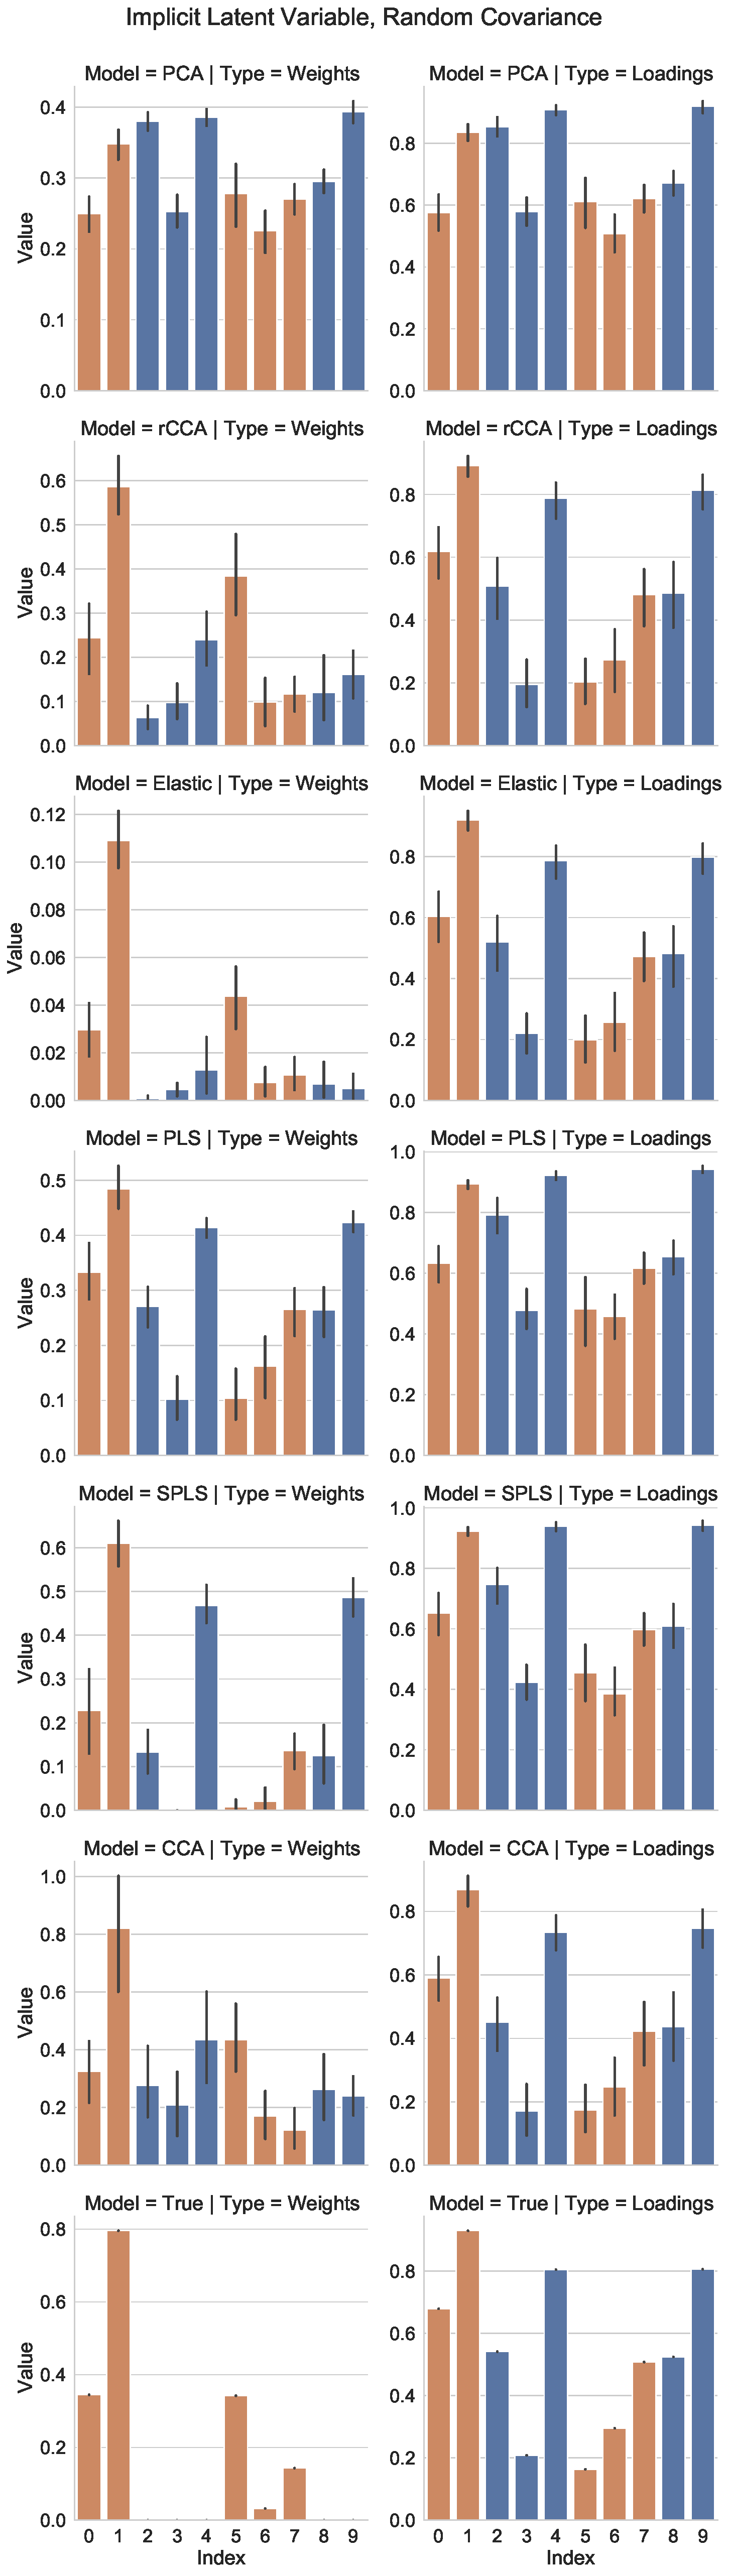
\includegraphics[width=\linewidth]{figures/simulated/low/Combined_Weights_Loadings_with_Error_Bars_Random_Covariance_implicit}
\caption{Random Covariance Matrices}
\end{subfigure}
\caption{Weights and Loadings for Implicit Latent Variable Data Generation.}
\end{figure}

\begin{figure}
\centering
\begin{subfigure}{0.49\linewidth}
\centering
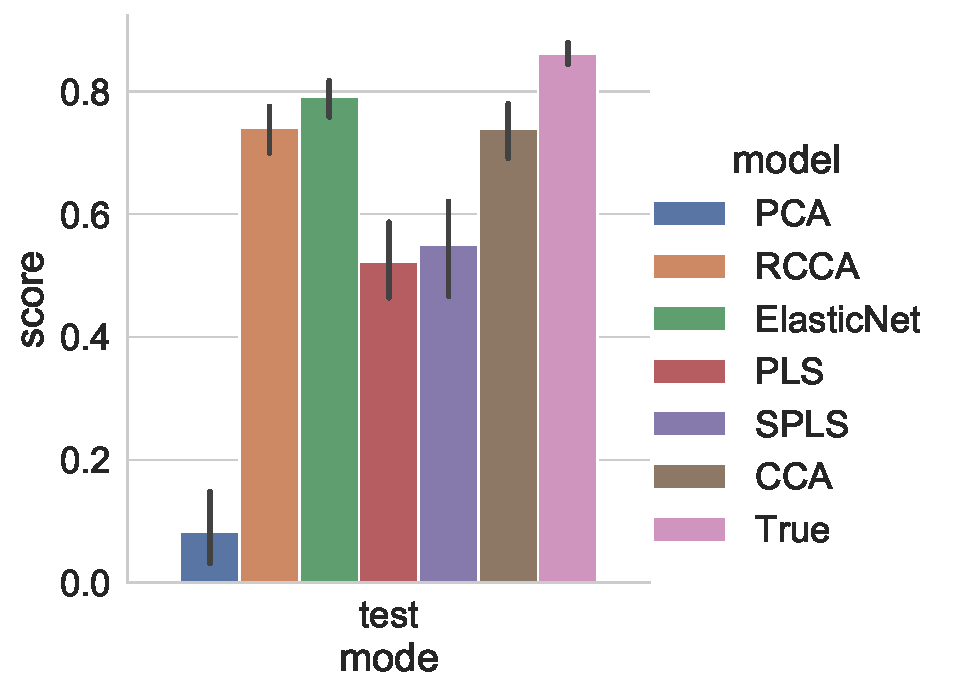
\includegraphics[width=\linewidth]{figures/simulated/low/Train_Test_Scores_Identity_Covariance_implicit}
\caption{Identity Covariance Matrices}
\end{subfigure}
%
\begin{subfigure}{0.49\linewidth}
\centering
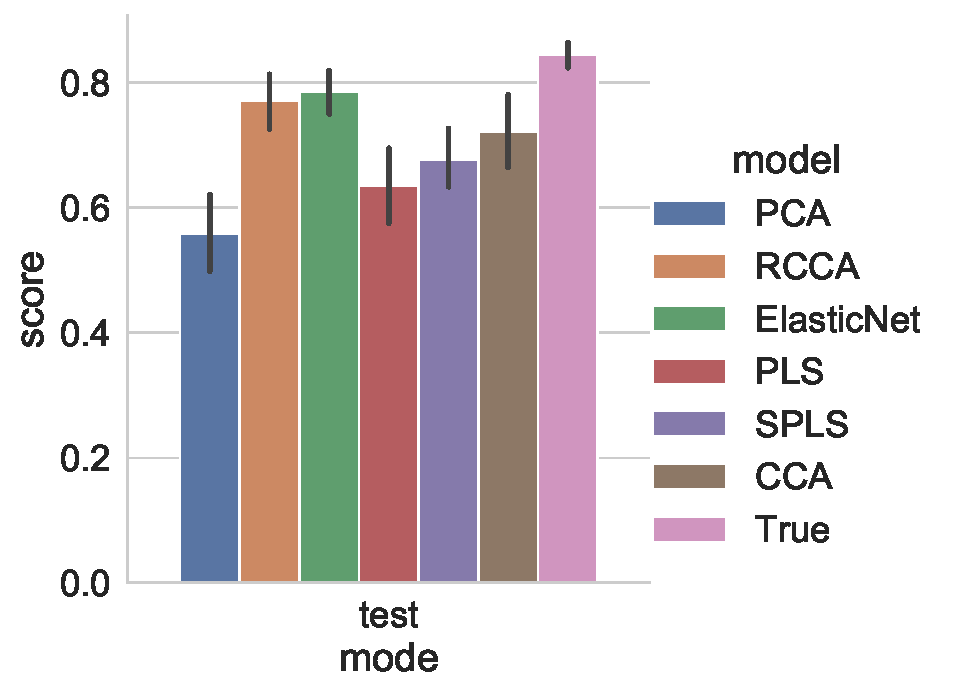
\includegraphics[width=\linewidth]{figures/simulated/low/Train_Test_Scores_Random_Covariance_implicit}
\caption{Random Covariance Matrices}
\end{subfigure}
\caption{Test Scores for Implicit Latent Variable Data Generation.}\label{fig:joint-scores}
\end{figure}

\paragraph{Explicit Latent Variables (Sparse Loadings):} A striking observation, though theoretically consistent, from Figure~\ref{fig:latent-variable-weights-loadings}a is that PCA almost perfectly recovers the true \gls{weights} and loadings for the \acrshort{gfa} model with identity noise covariance.
Admittedly, we have chosen a reasonably high signal-to-noise ratio for this experiment, but this nonetheless demonstrates that PCA can be a useful baseline for multiview data under an isotropic latent variable noise model.
Indeed, in the identity noise covariance scenario, all the models perform similarly (Figure~\ref{fig:latent-variable-scores}a) with the exception of \acrshort{cca} which appears to be unstable in this setting (Figure~\ref{fig:latent-variable-weights-loadings}a).
In the random noise covariance scenario, PCA performs poorly, and \acrshort{cca} now performs well (Figure~\ref{fig:latent-variable-scores}b).
Figure~\ref{fig:latent-variable-weights-loadings}b indicates that with anisotropic noise covariance, PCA no longer captures the true loadings.
There is no strong evidence that \acrshort{spls} or Elastic Net regularization outperform \acrshort{pls} or \acrshort{rcca}, respectively, in this setting.
This is unsurprising because the true \gls{weights} are not sparse, and so the additional sparsity constraints do not help.
However, this does illustrate that priors on \gls{weights} do not translate well to priors on loadings.

\begin{figure}
\centering
\begin{subfigure}{0.49\linewidth}
\centering
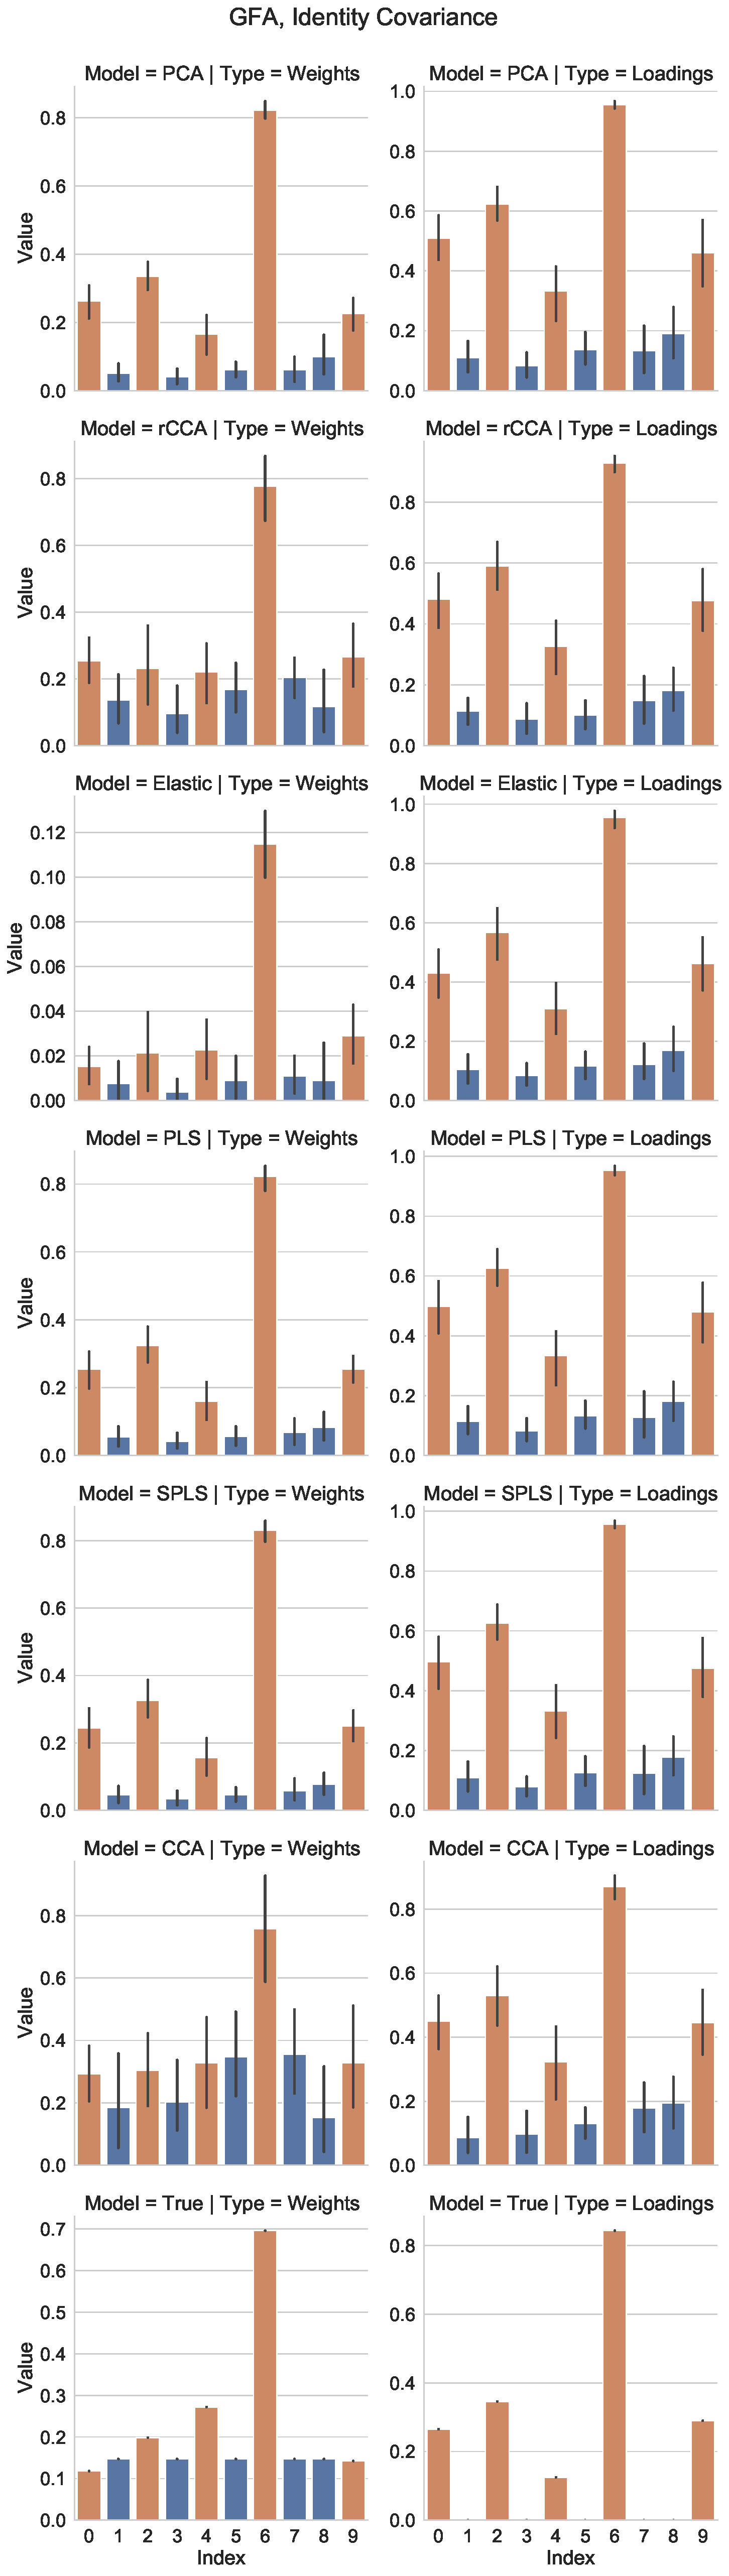
\includegraphics[width=\linewidth]{figures/simulated/low/Combined_Weights_Loadings_with_Error_Bars_Identity_Covariance_explicit}
\caption{\acrshort{gfa} (Identity Noise)}
\end{subfigure}
%
\begin{subfigure}{0.49\linewidth}
\centering
\includegraphics[width=\linewidth]{figures/simulated/low/Combined_Weights_Loadings_with_Error_Bars_Random_Covariance_explicit}
\caption{Probabilistic \acrshort{cca} (Random Noise)}
\end{subfigure}
\caption{Weights and Loadings for Explicit Latent Variable Data Generation Models.}\label{fig:latent-variable-weights-loadings}
\end{figure}

\begin{figure}
\centering
\begin{subfigure}{0.49\linewidth}
\centering
\includegraphics[width=\linewidth]{figures/simulated/low/Train_Test_Scores_Identity_Covariance_explicit}
\caption{\acrshort{gfa}}
\end{subfigure}
%
\begin{subfigure}{0.49\linewidth}
\centering
\includegraphics[width=\linewidth]{figures/simulated/low/Train_Test_Scores_Random_Covariance_explicit}
\caption{Probabilistic \acrshort{cca}}
\end{subfigure}
\caption{Test Scores for Explicit Latent Variable Data Generation Models.}\label{fig:latent-variable-scores}
\end{figure}

\paragraph{Measuring the Identitiness of the Covariance Matrices}
The theory we developed in section~\ref{subsec:generative-perspectives} suggests that the identitiness of the covariance matrices is crucial for understanding how imposing sparsity on the \gls{weights} imposes a prior belief in sparsity on the more biologically interesting loadings.
We can measure the identitiness of the covariance matrices by looking at the eigenvalues of the covariance matrices.
If the eigenvalues of the sample covariance matrix are all close to 1, then the sample covariance matrix is close to identity.
Departures from 1 indicate that the sample covariance matrix is not close to identity and imply multicollinearity in the data.

In the simulated data, we can see that the data generation models with identity noise covariance matrices, have eigenvalues closer to one than (Figure~\ref{fig:covariance-eigenvalues-simulated-low}).
On the other hand, these plots (shown for 10 random samples) show that all of the sample covariance matrices depart from the ideal case, \textit{even when the true covariance matrices are identity}.

\begin{figure}
\centering
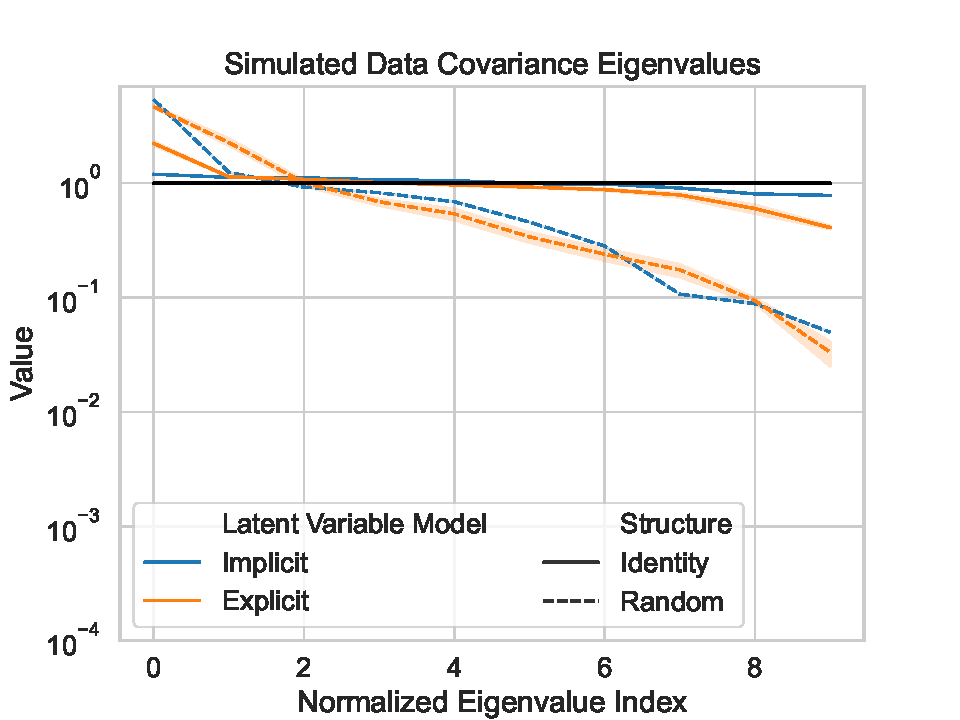
\includegraphics[width=0.8\linewidth]{figures/covariance/simulated_covariance_eigenvalues_low}
\caption{Eigenvalues of the covariance matrices for the simulated datasets.}\label{fig:covariance-eigenvalues-simulated-low}
\end{figure}


\subsection{Repeated Columns}\label{subsec:repeated-columns}

In this section, we explore the stability of \gls{weights} and \gls{loadings} in \acrshort{cca} models when faced with repeated columns in the data.
Our theoretical analysis suggests that while \gls{weights} may vary and are arbitrary with repeated columns, \gls{loadings}  remain consistent.

\begin{figure}
\centering
\begin{subfigure}{0.49\linewidth}
\centering
\includegraphics[width=\linewidth]{figures/simulated/repeated/Combined_Weights_Loadings_with_Error_Bars_Identity_Covariance_implicit}
\caption{Identity Covariance Matrices}
\end{subfigure}
%
\begin{subfigure}{0.49\linewidth}
\centering
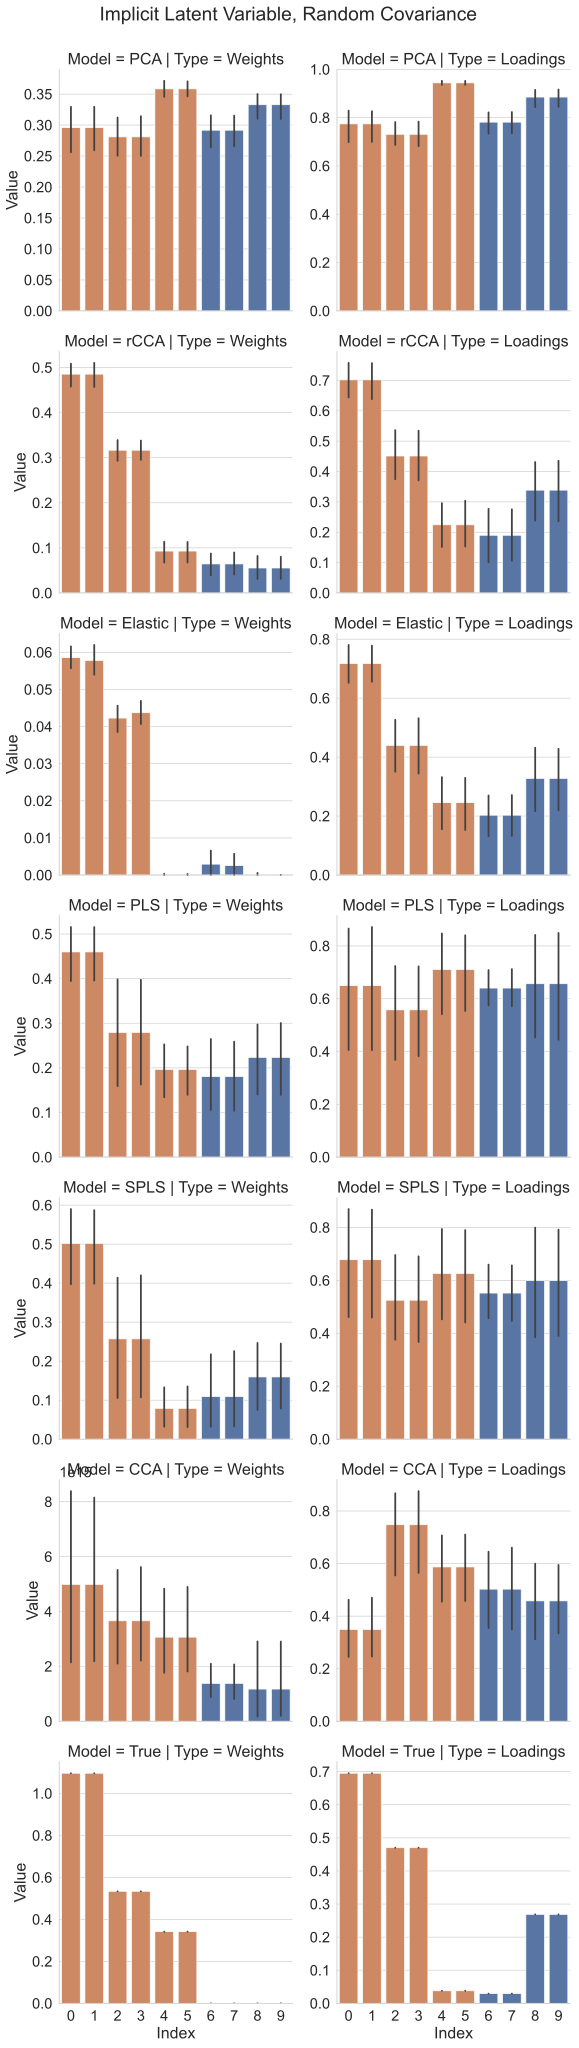
\includegraphics[width=\linewidth]{figures/simulated/repeated/Combined_Weights_Loadings_with_Error_Bars_Random_Covariance_implicit}
\caption{Random Covariance Matrices}
\end{subfigure}
\caption{Weights and Loadings for Implicit Latent Variable Data Generation.}
\end{figure}

\begin{figure}
\centering
\begin{subfigure}{0.49\linewidth}
\centering
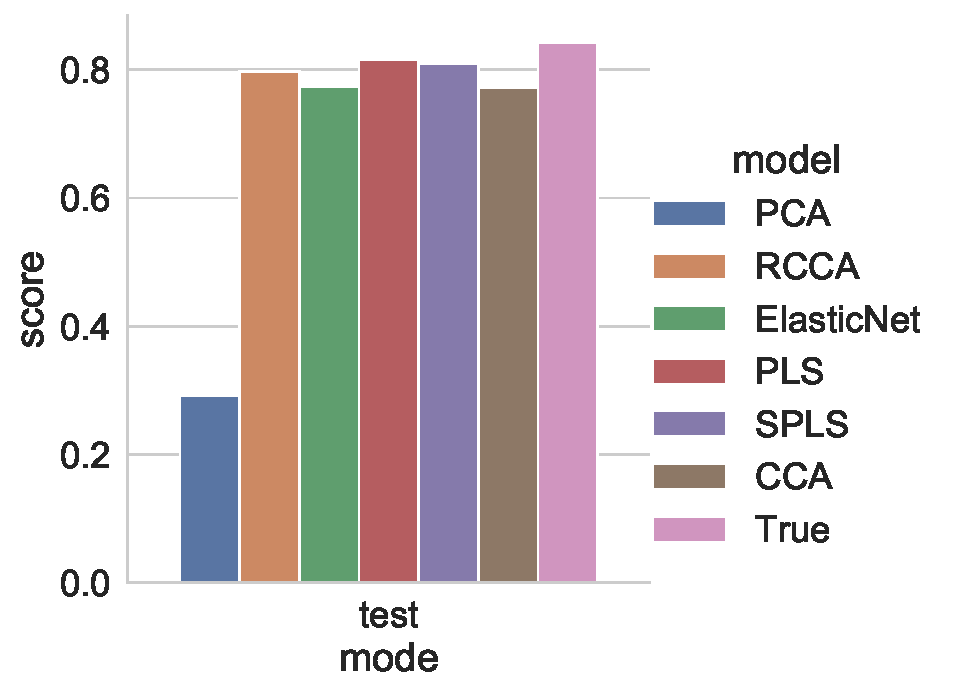
\includegraphics[width=\linewidth]{figures/simulated/repeated/Train_Test_Scores_Identity_Covariance_implicit}
\caption{Identity Covariance Matrices}
\end{subfigure}
\end{figure}

Empirical results from our experiments validate this theoretical proposition.
We observed that in \acrshort{pls} and \acrshort{spls} models, which are significantly regularized (L2 regularization), the \gls{weights} for repeated features tend to be uniform.
However, in the case of \acrshort{cca} the \gls{weights} applied to repeated features are almost completely arbitrary (see the scale).
For Elastic and Ridge \acrshort{cca}, the \gls{weights} applied to repeated features, though not identical, display greater stability due to shrinkage effects.
In contrast, \gls{loadings} for repeated features remained consistent across all tested models, reinforcing our theoretical stance on their preferential use for model interpretation in scenarios with repeated columns or near-repeated columns.

%

%\subsection{High-Dimensional Simulated Data}
%In this section we consider only the latent variable models in order to ensure we have a sufficient signal-to-noise ratio to compare the models as we are deliberately undersampled.
%Figure~\ref{fig:latent-variable-weights-loadings-high}a once again shows that PCA is a useful baseline for multiview data under an isotropic noise model, even in the high-dimensional setting.
%On the other hand, \acrshort{cca} cannot recover any signal when it is overparameterized.
%Ridge \acrshort{cca} and \acrshort{pls} perform similarly, perhaps because the only identifiable signal is the \acrshort{pls} signal (since the \acrshort{cca} signal is not identifiable).
%Figure~\ref{fig:latent-variable-weights-loadings-high}b illustrates clearly that both \acrshort{rcca} and ElasticNet with their tunable L2 regularization both outperform \acrshort{pls} and \acrshort{spls} with fixed and maximal L2 regularization.
%It appears that in high dimensions correlated noise is a significant problem for \acrshort{pls} (and therefore \acrshort{spls}) when used as regularized \acrshort{cca} models, even though the models are identifiable.
%
%\begin{figure}
%\centering
%\begin{subfigure}{0.49\linewidth}
%\centering
%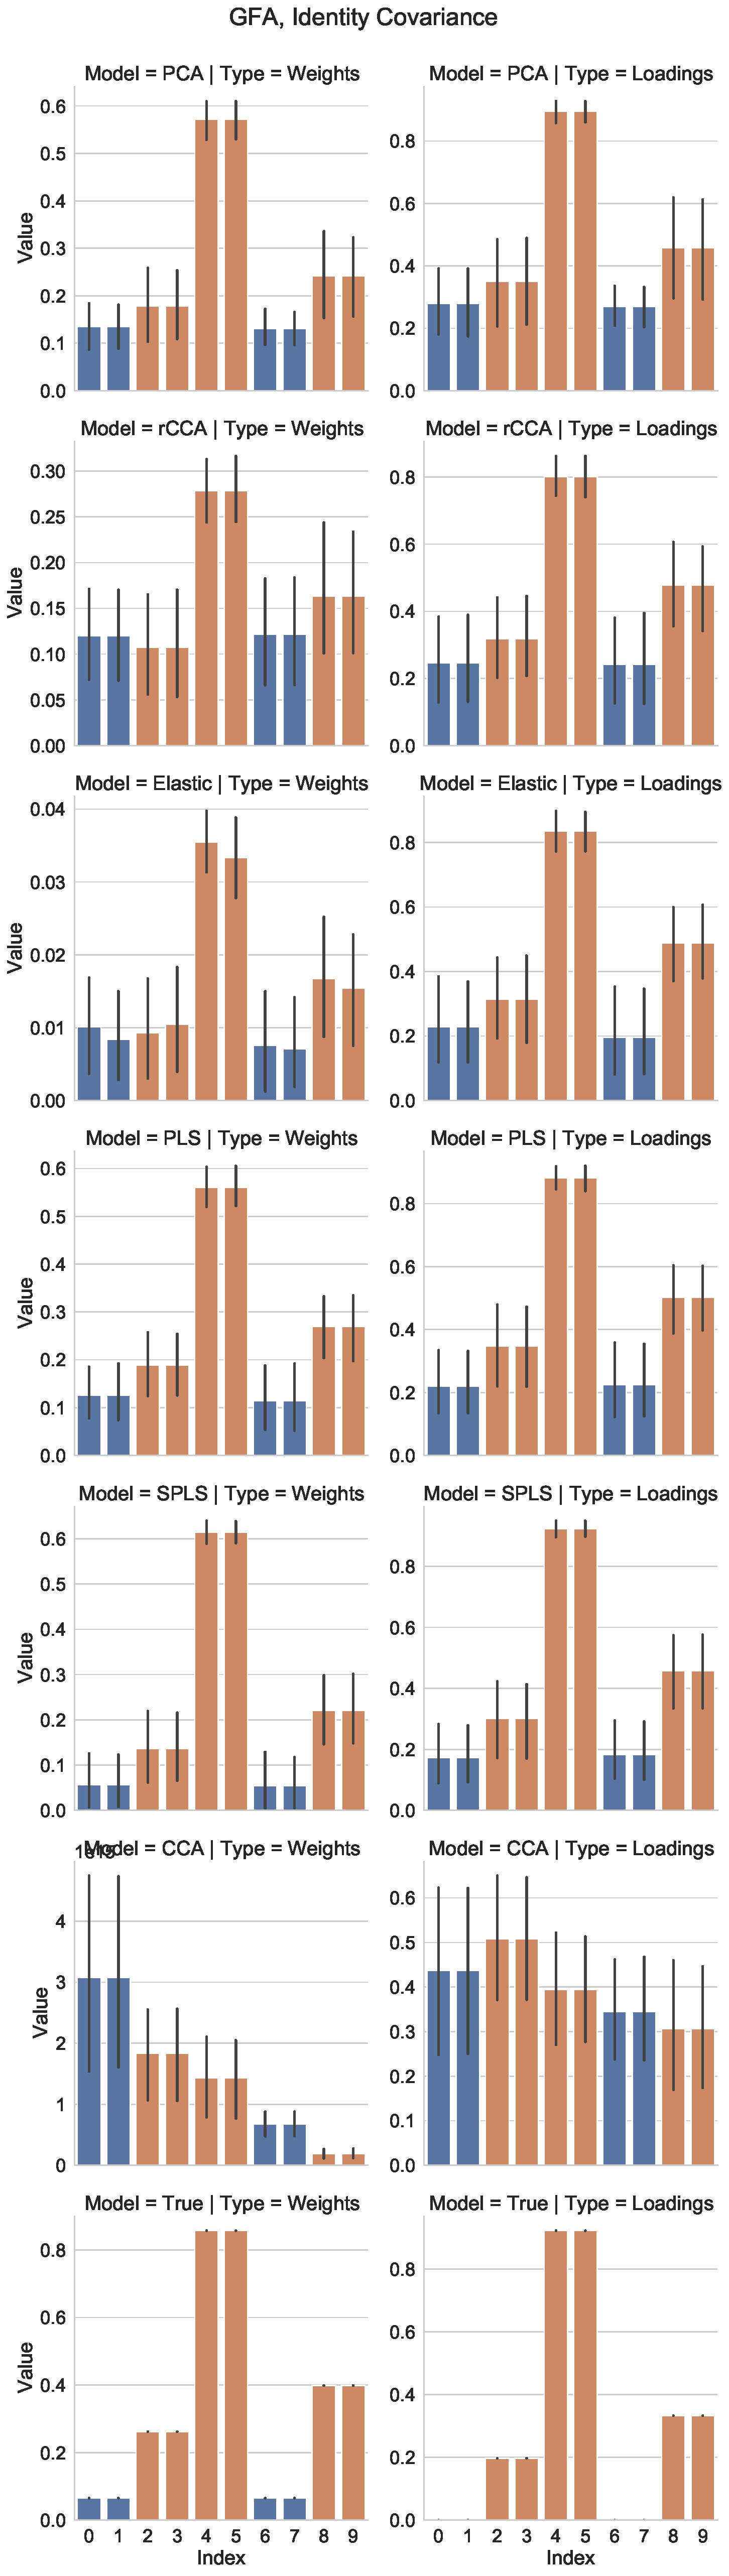
\includegraphics[width=\linewidth]{figures/simulated/high/Combined_Weights_Loadings_with_Error_Bars_Identity_Covariance_explicit}
%\caption{Identity Covariance Latent Variable}
%\end{subfigure}
%%
%\begin{subfigure}{0.49\linewidth}
%\centering
%\includegraphics[width=\linewidth]{figures/simulated/high/Combined_Weights_Loadings_with_Error_Bars_Random_Covariance_explicit}
%\caption{Random Covariance Latent Variable}
%\end{subfigure}
%\caption{Weights and Loadings for High-Dimensional Explicit Latent Variable Data Generation.}\label{fig:latent-variable-weights-loadings-high}
%\end{figure}
%
%\begin{figure}
%\centering
%\begin{subfigure}{0.49\linewidth}
%\centering
%\includegraphics[width=\linewidth]{figures/simulated/high/Train_Test_Scores_Identity_Covariance_explicit}
%\caption{}
%\end{subfigure}
%%
%\begin{subfigure}{0.49\linewidth}
%\centering
%\includegraphics[width=\linewidth]{figures/simulated/high/Train_Test_Scores_Random_Covariance_explicit}
%\caption{}
%\end{subfigure}
%\caption{Test Scores for High-Dimensional Explicit Latent Variable Data Generation Models.}\label{fig:latent-variable-scores-high}
%\end{figure}

%\paragraph{Identitiness of the Covariance Matrices}
%
%As in the low-dimensional case, we can measure the identitiness of the covariance matrices by looking at the eigenvalues of the covariance matrices.
%
%\begin{figure}
%\centering
%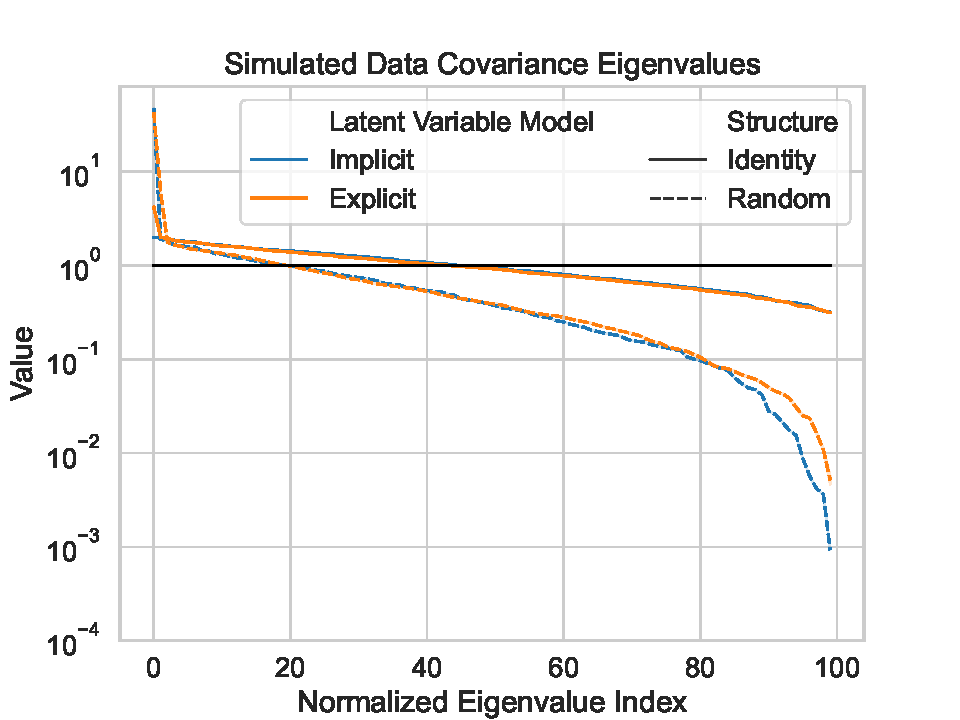
\includegraphics[width=0.8\linewidth]{figures/covariance/simulated_covariance_eigenvalues_high}
%\caption{Eigenvalues of the covariance matrices for the simulated datasets.}\label{fig:covariance-eigenvalues-simulated-high}
%\end{figure}

\newpage
\subsection{Human Connectome Project (\acrshort{hcp}) Data}

Next, we revisit the results from the previous chapter on the \acrshort{hcp} data.
However this time we focus on the \gls{loadings} rather than the weights.

\subsubsection{Behaviour Weights and Loadings}



\begin{figure}
\centering
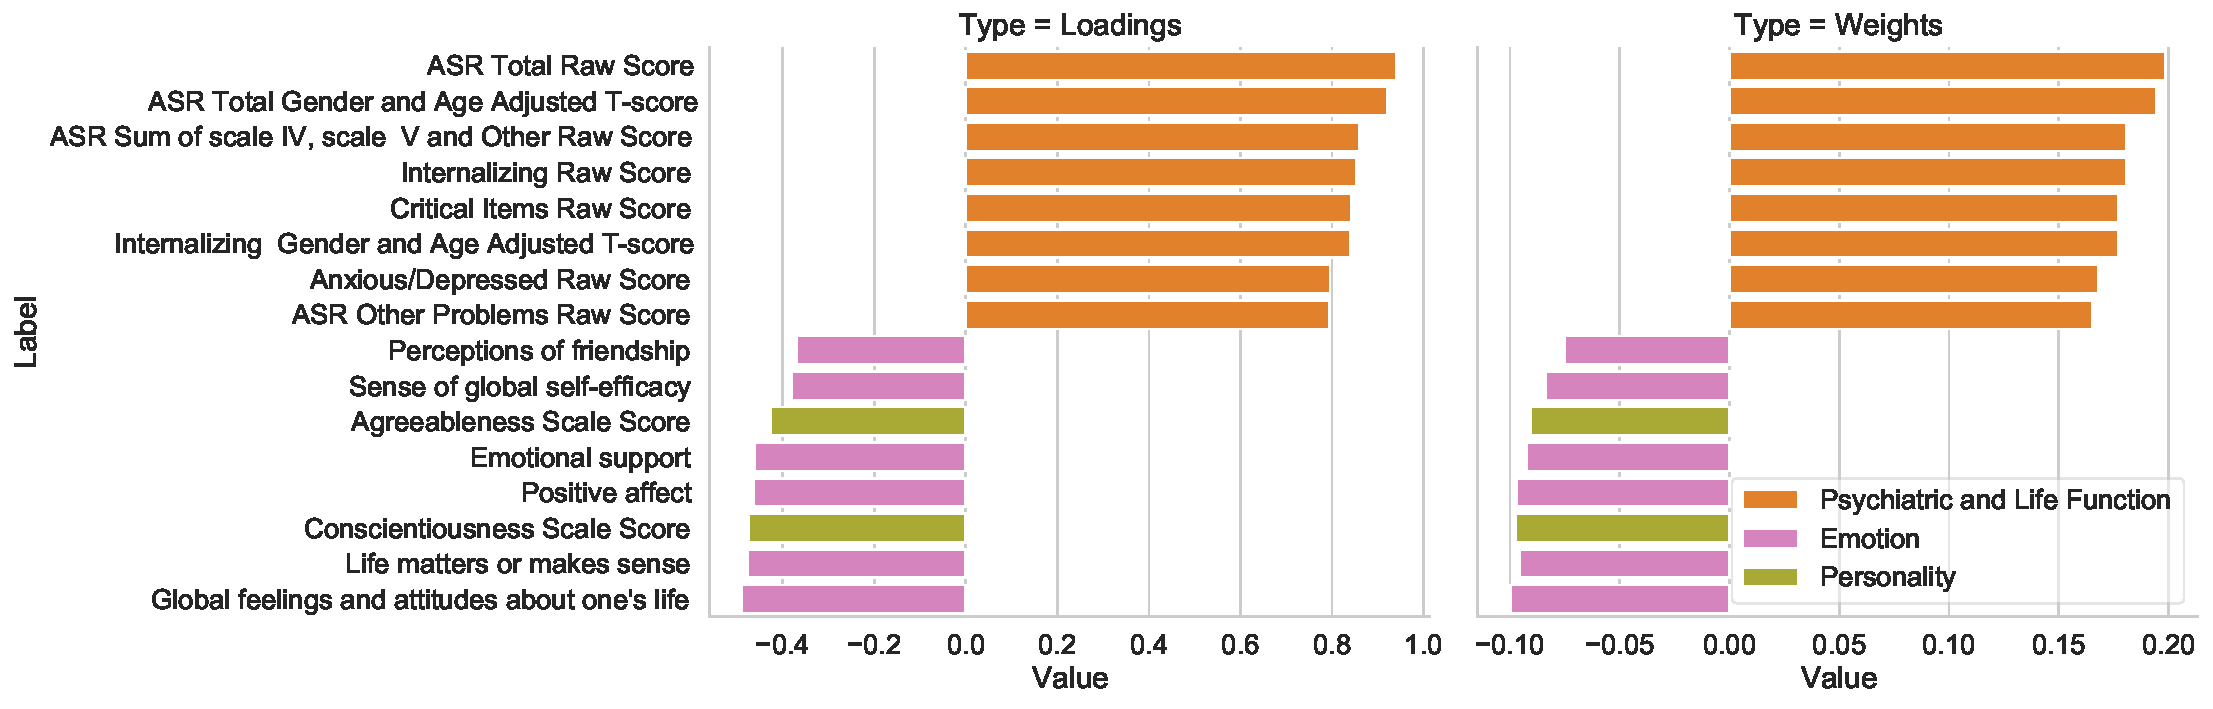
\includegraphics[width=0.8\linewidth]{figures/hcp/PCA behaviour weights and loadings}
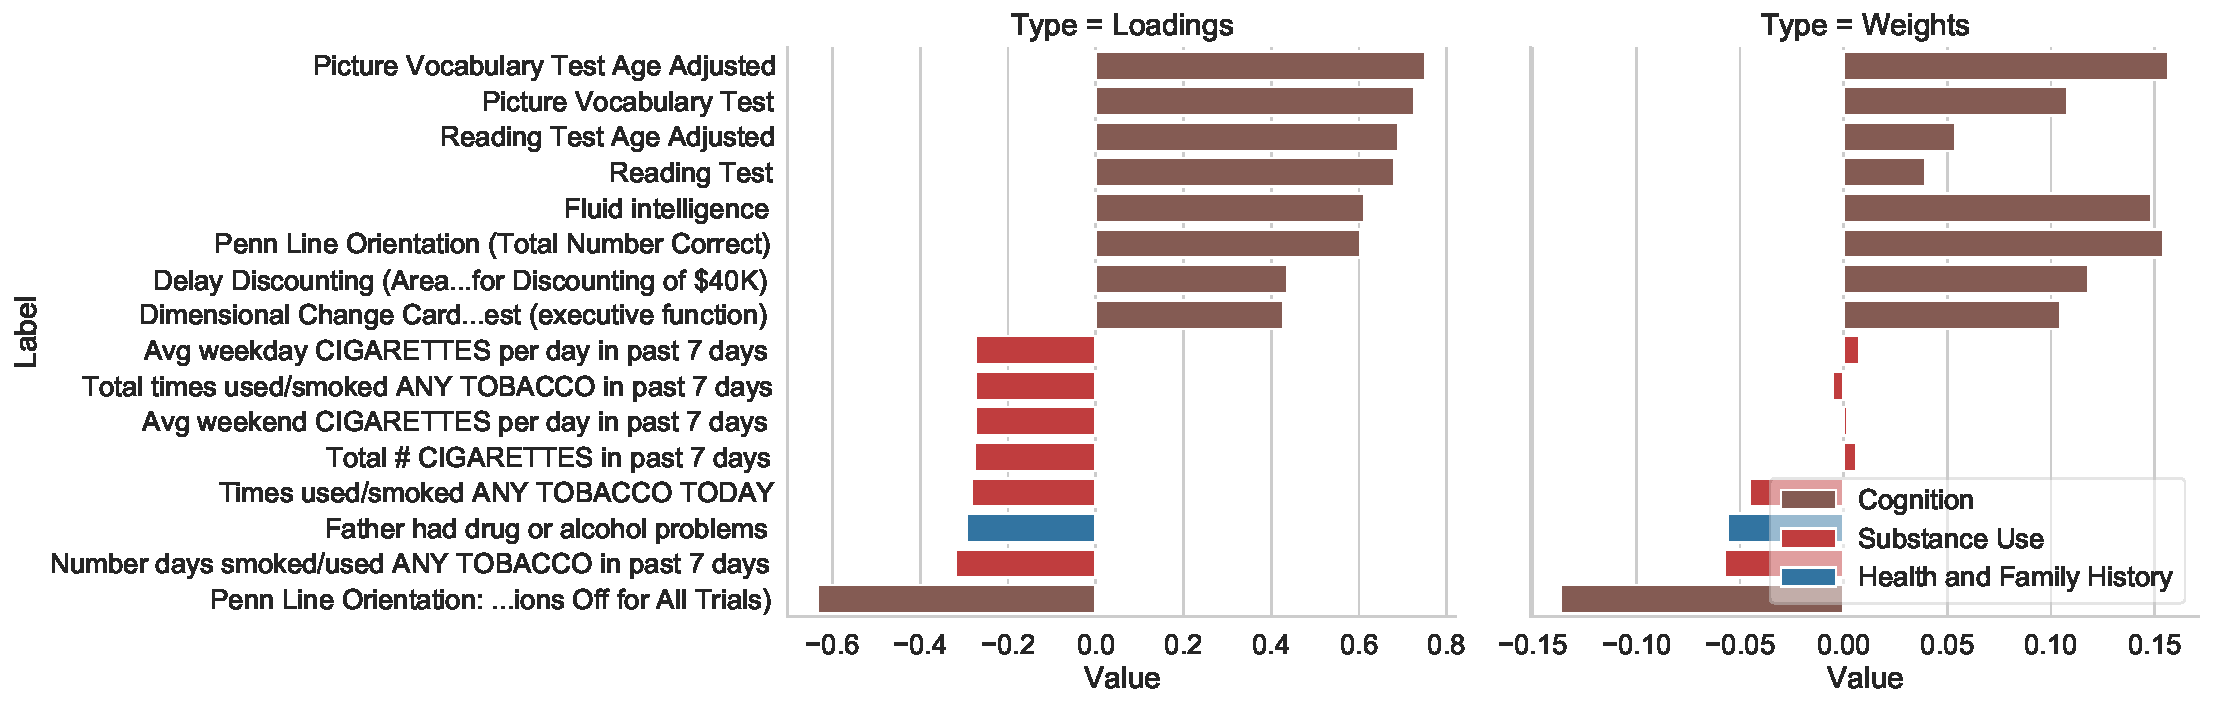
\includegraphics[width=0.8\linewidth]{figures/hcp/RCCA behaviour weights and loadings}
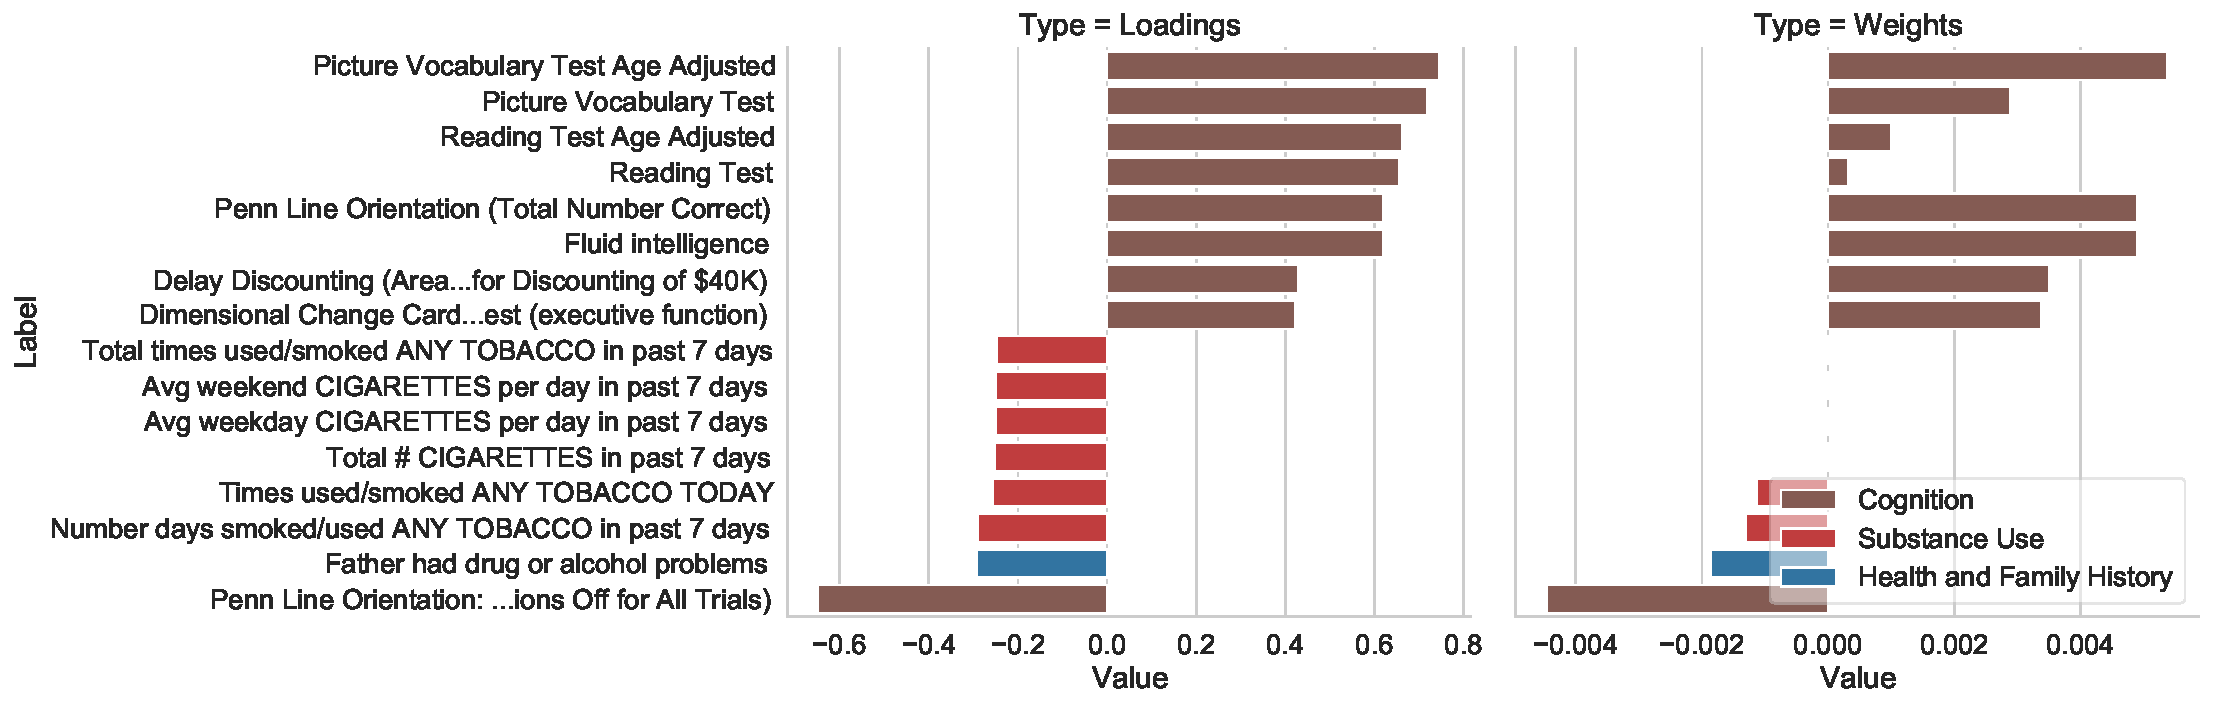
\includegraphics[width=0.8\linewidth]{figures/hcp/ElasticNet behaviour weights and loadings}
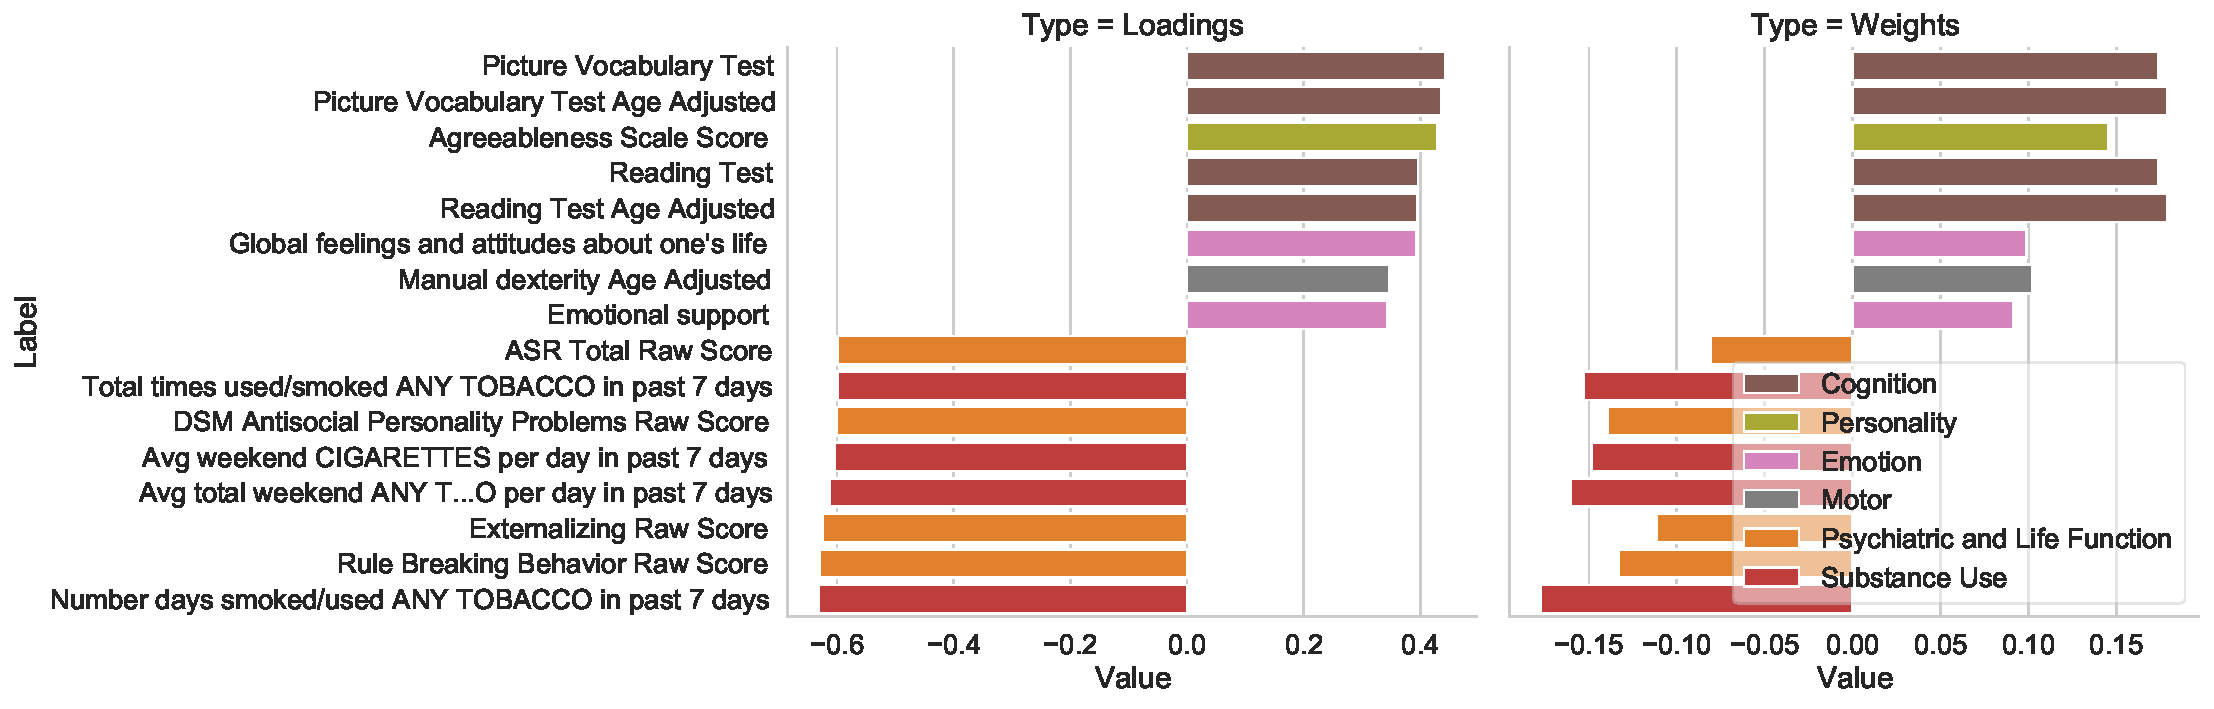
\includegraphics[width=0.8\linewidth]{figures/hcp/PLS behaviour weights and loadings}
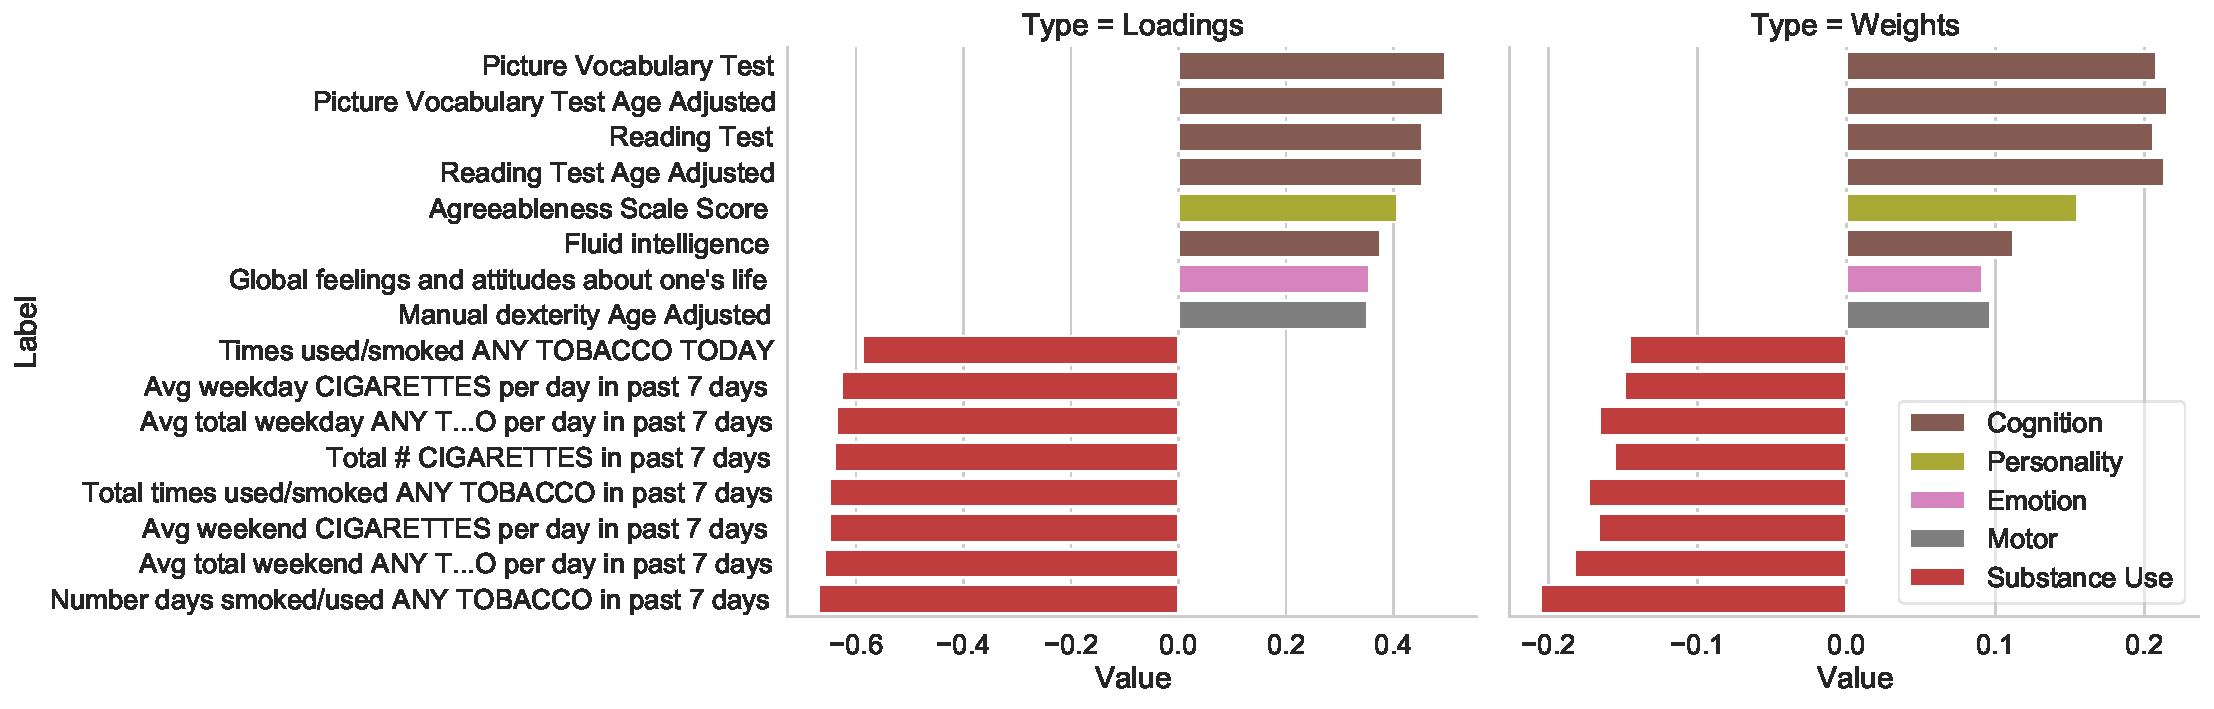
\includegraphics[width=0.8\linewidth]{figures/hcp/SPLS behaviour weights and loadings}
\caption{Top 8 positive and negative non-imaging \gls{loadings} for each model}
\end{figure}

\subsubsection{Brain Connectivity Weights and Loadings}

\begin{figure}
\centering
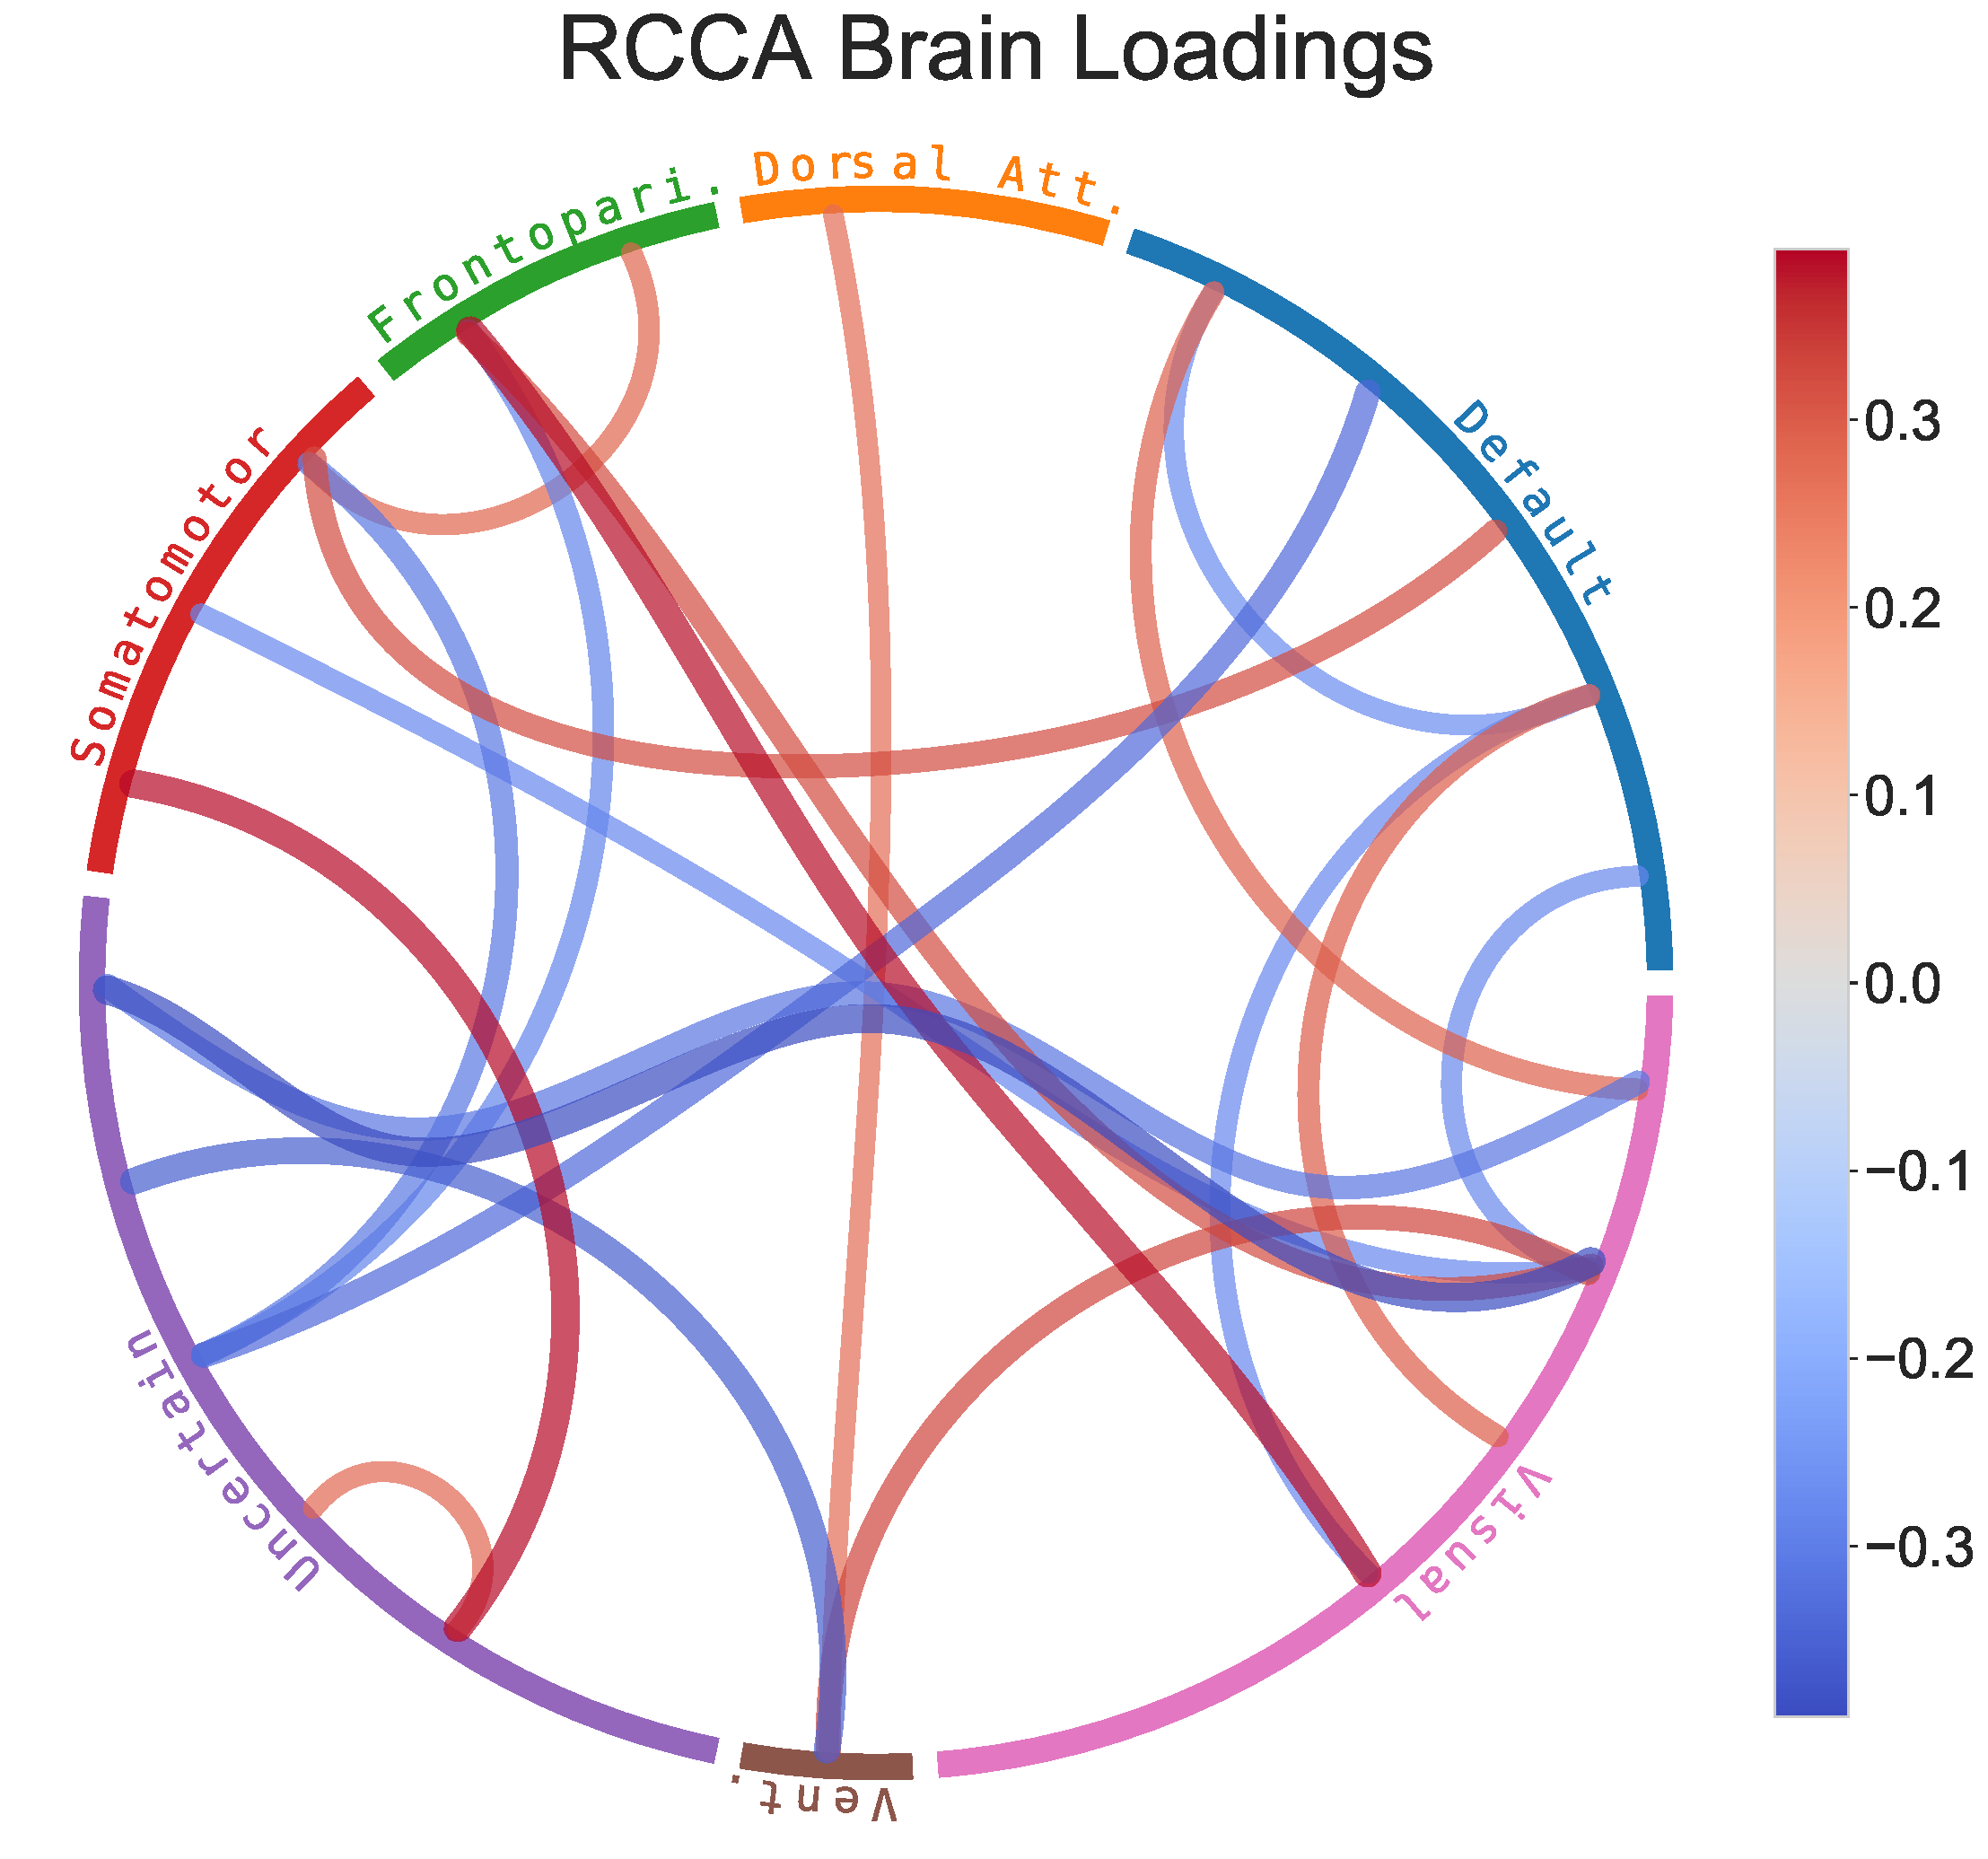
\includegraphics[width=0.49\linewidth]{figures/hcp/RCCA brain loadings}
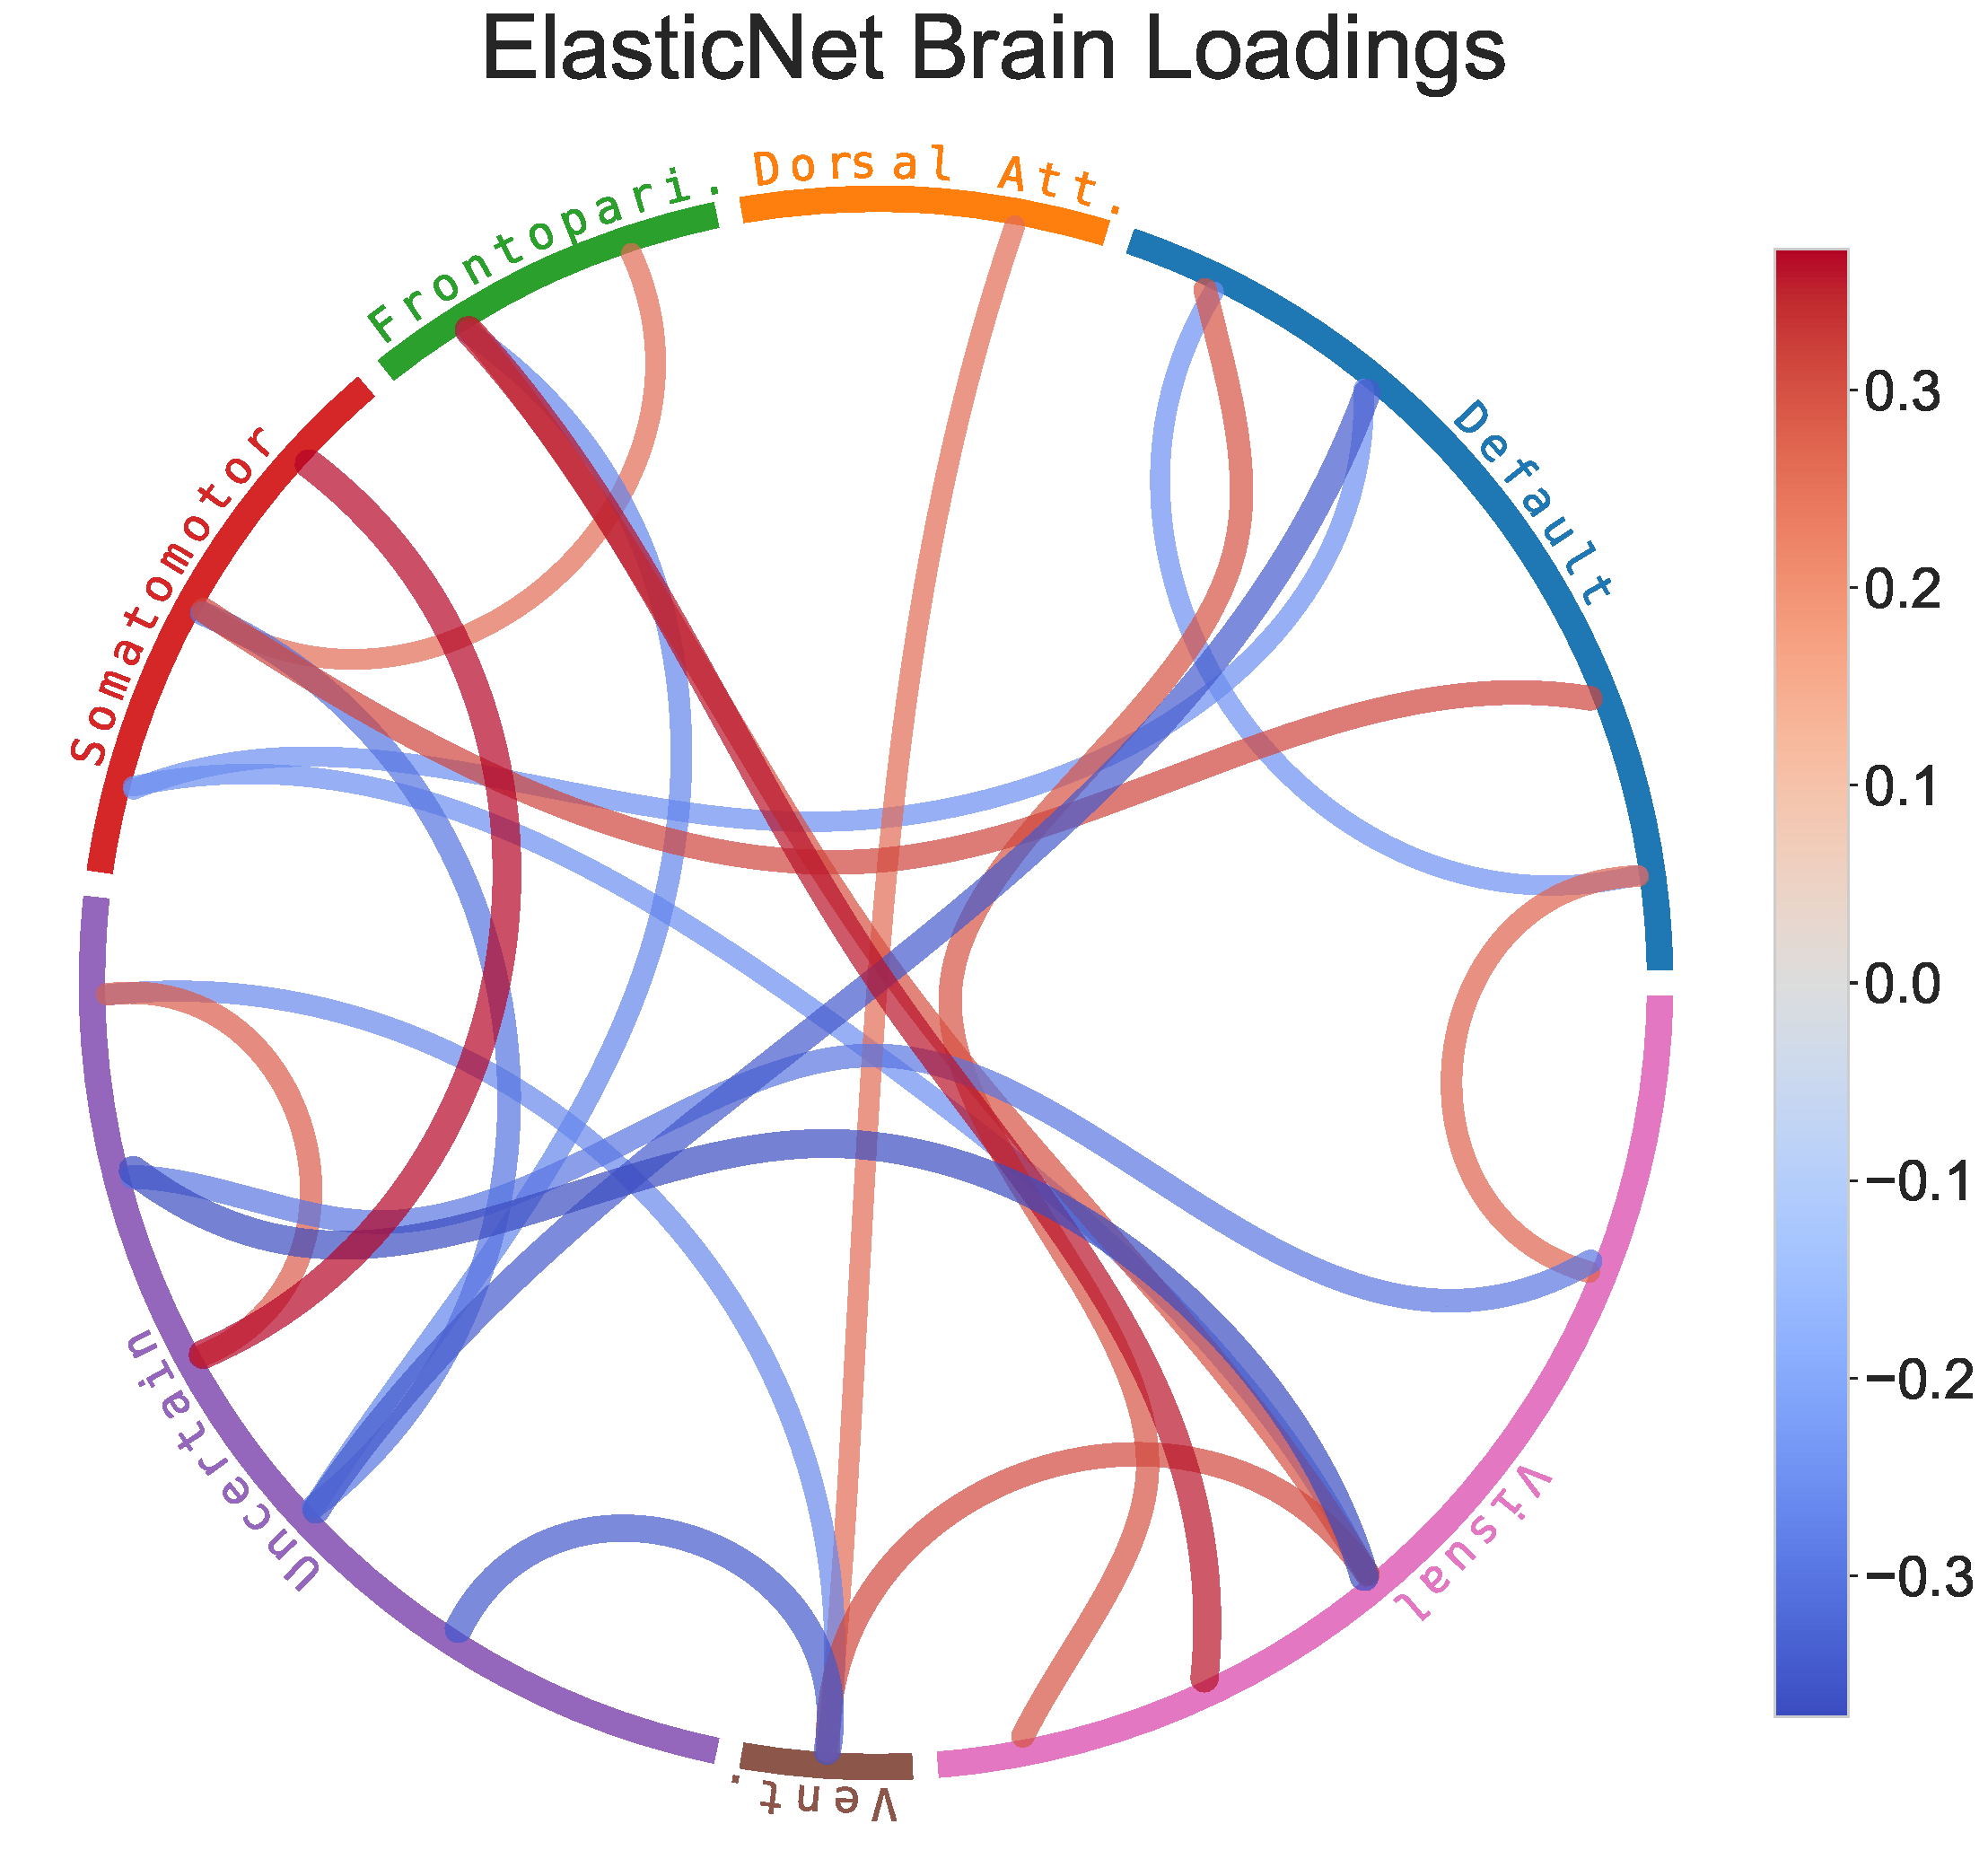
\includegraphics[width=0.49\linewidth]{figures/hcp/ElasticNet brain loadings}
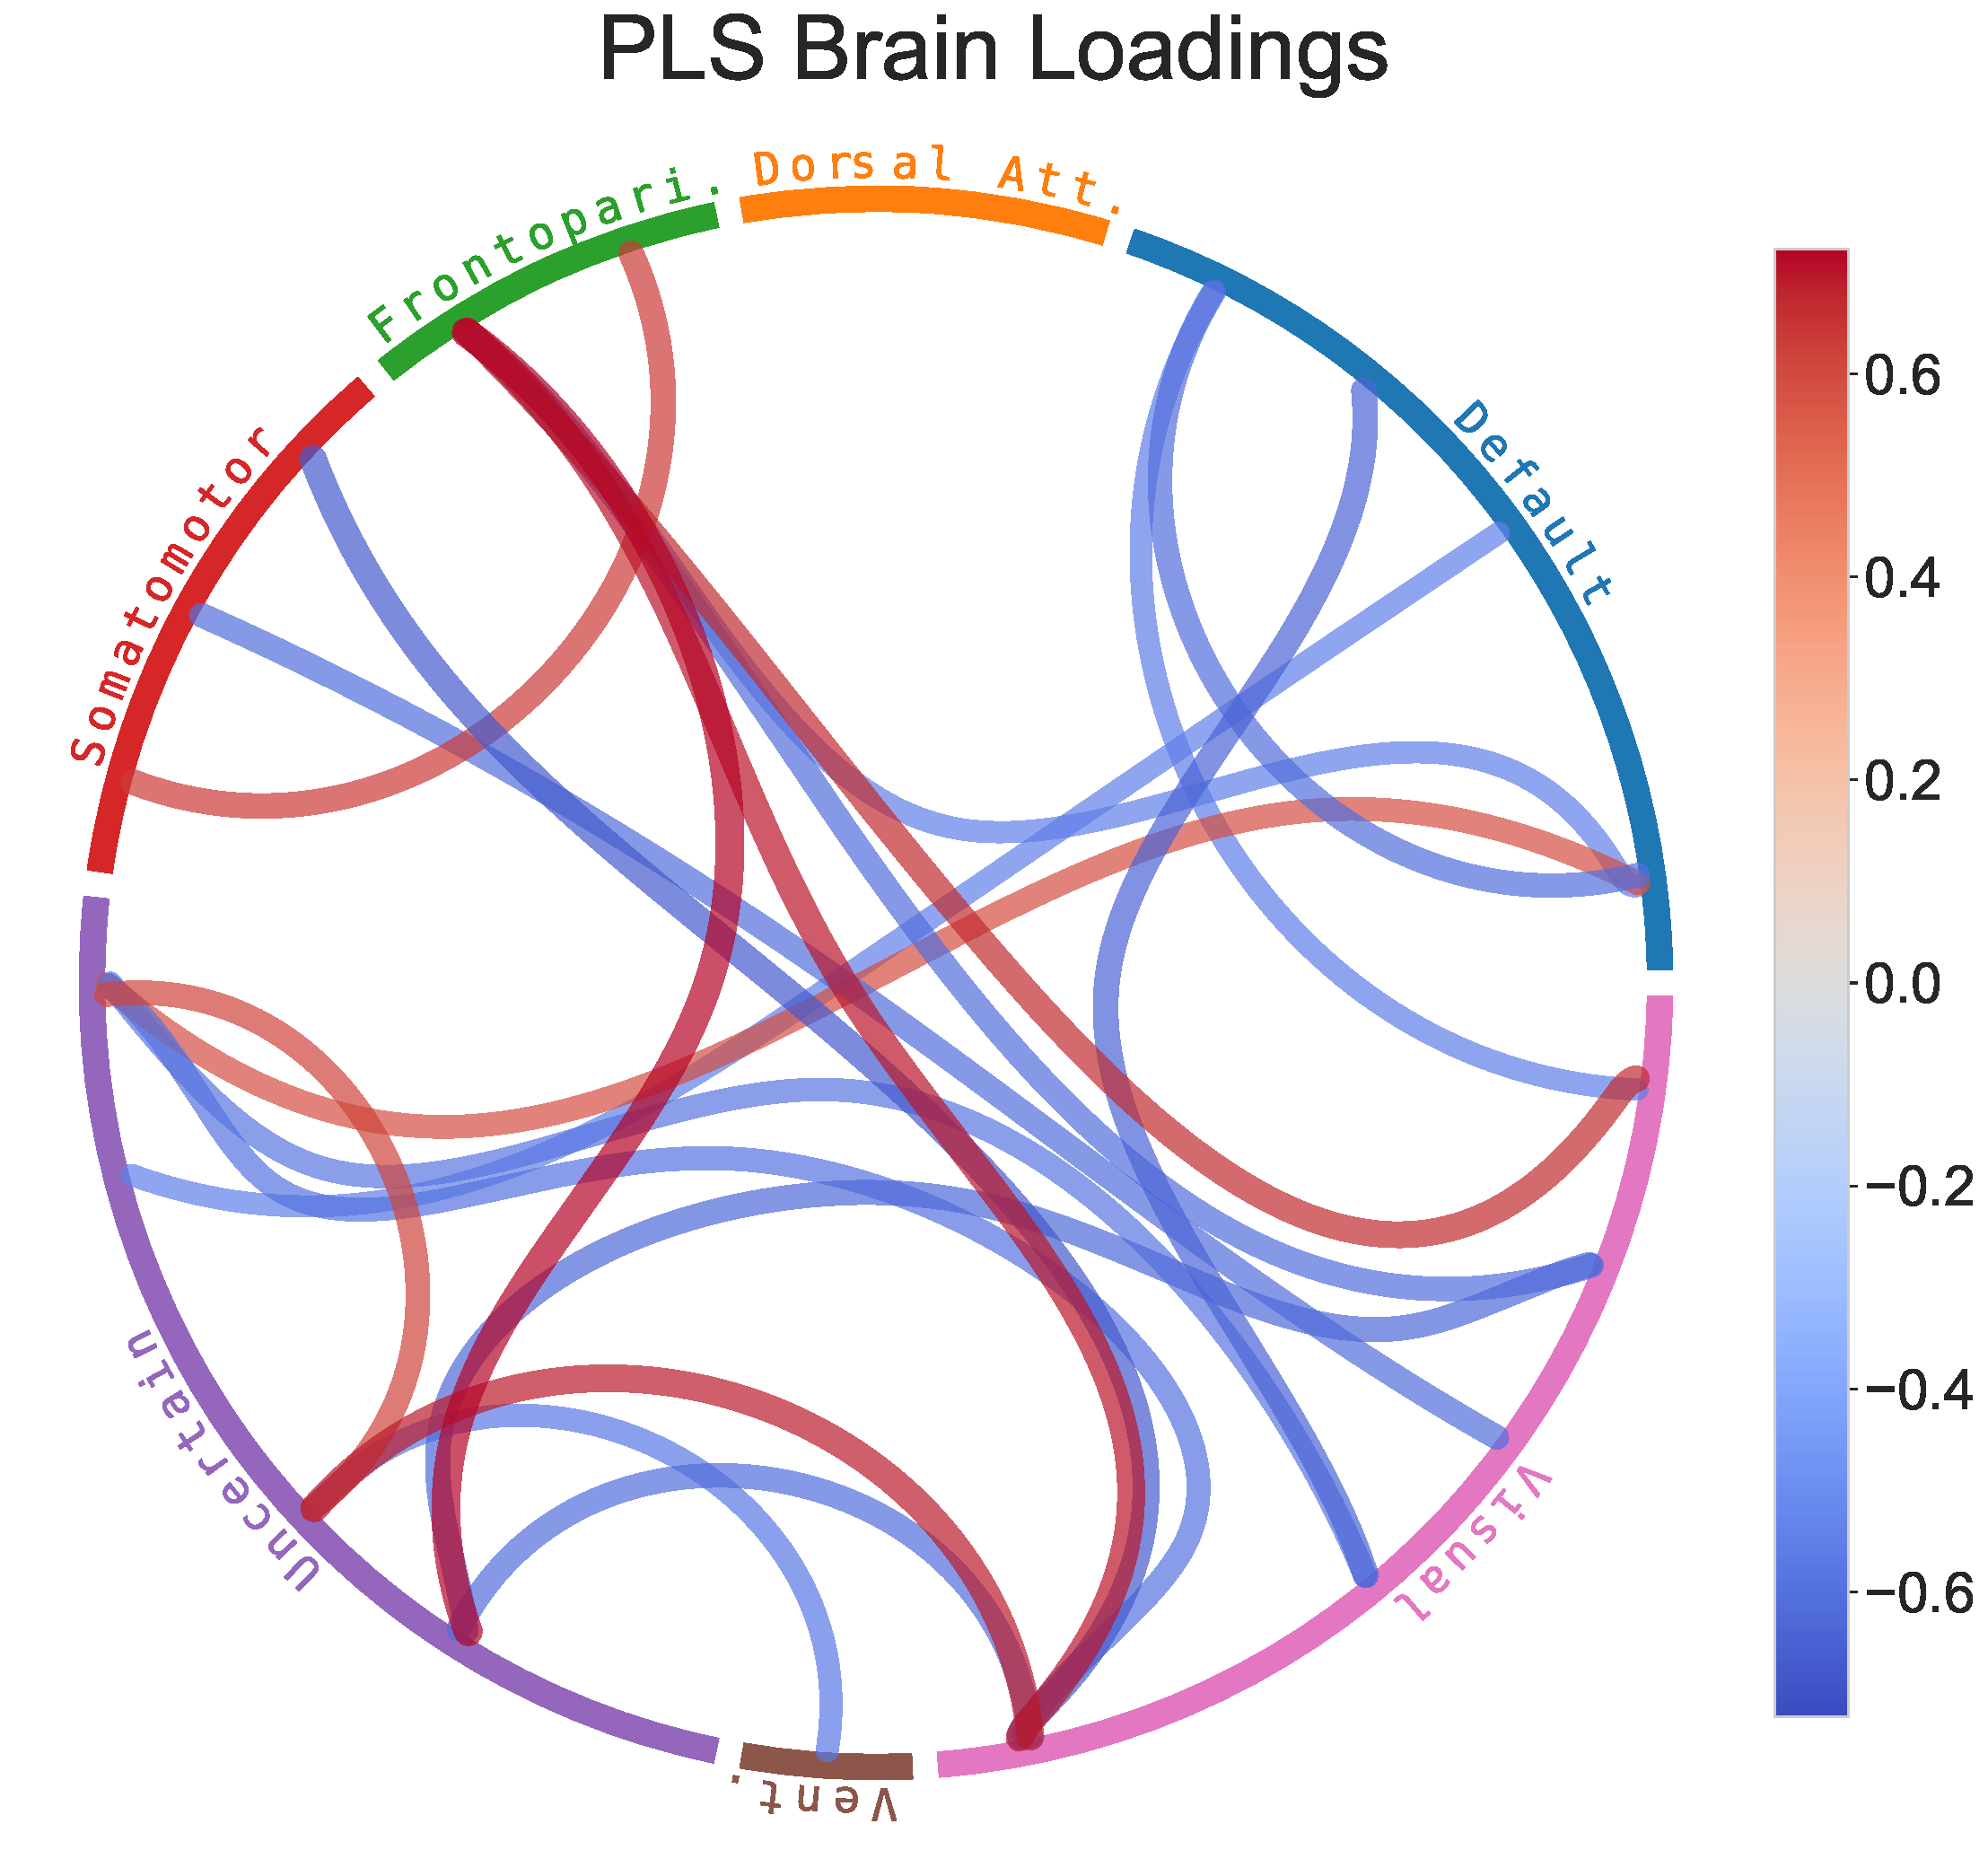
\includegraphics[width=0.49\linewidth]{figures/hcp/PLS brain loadings}
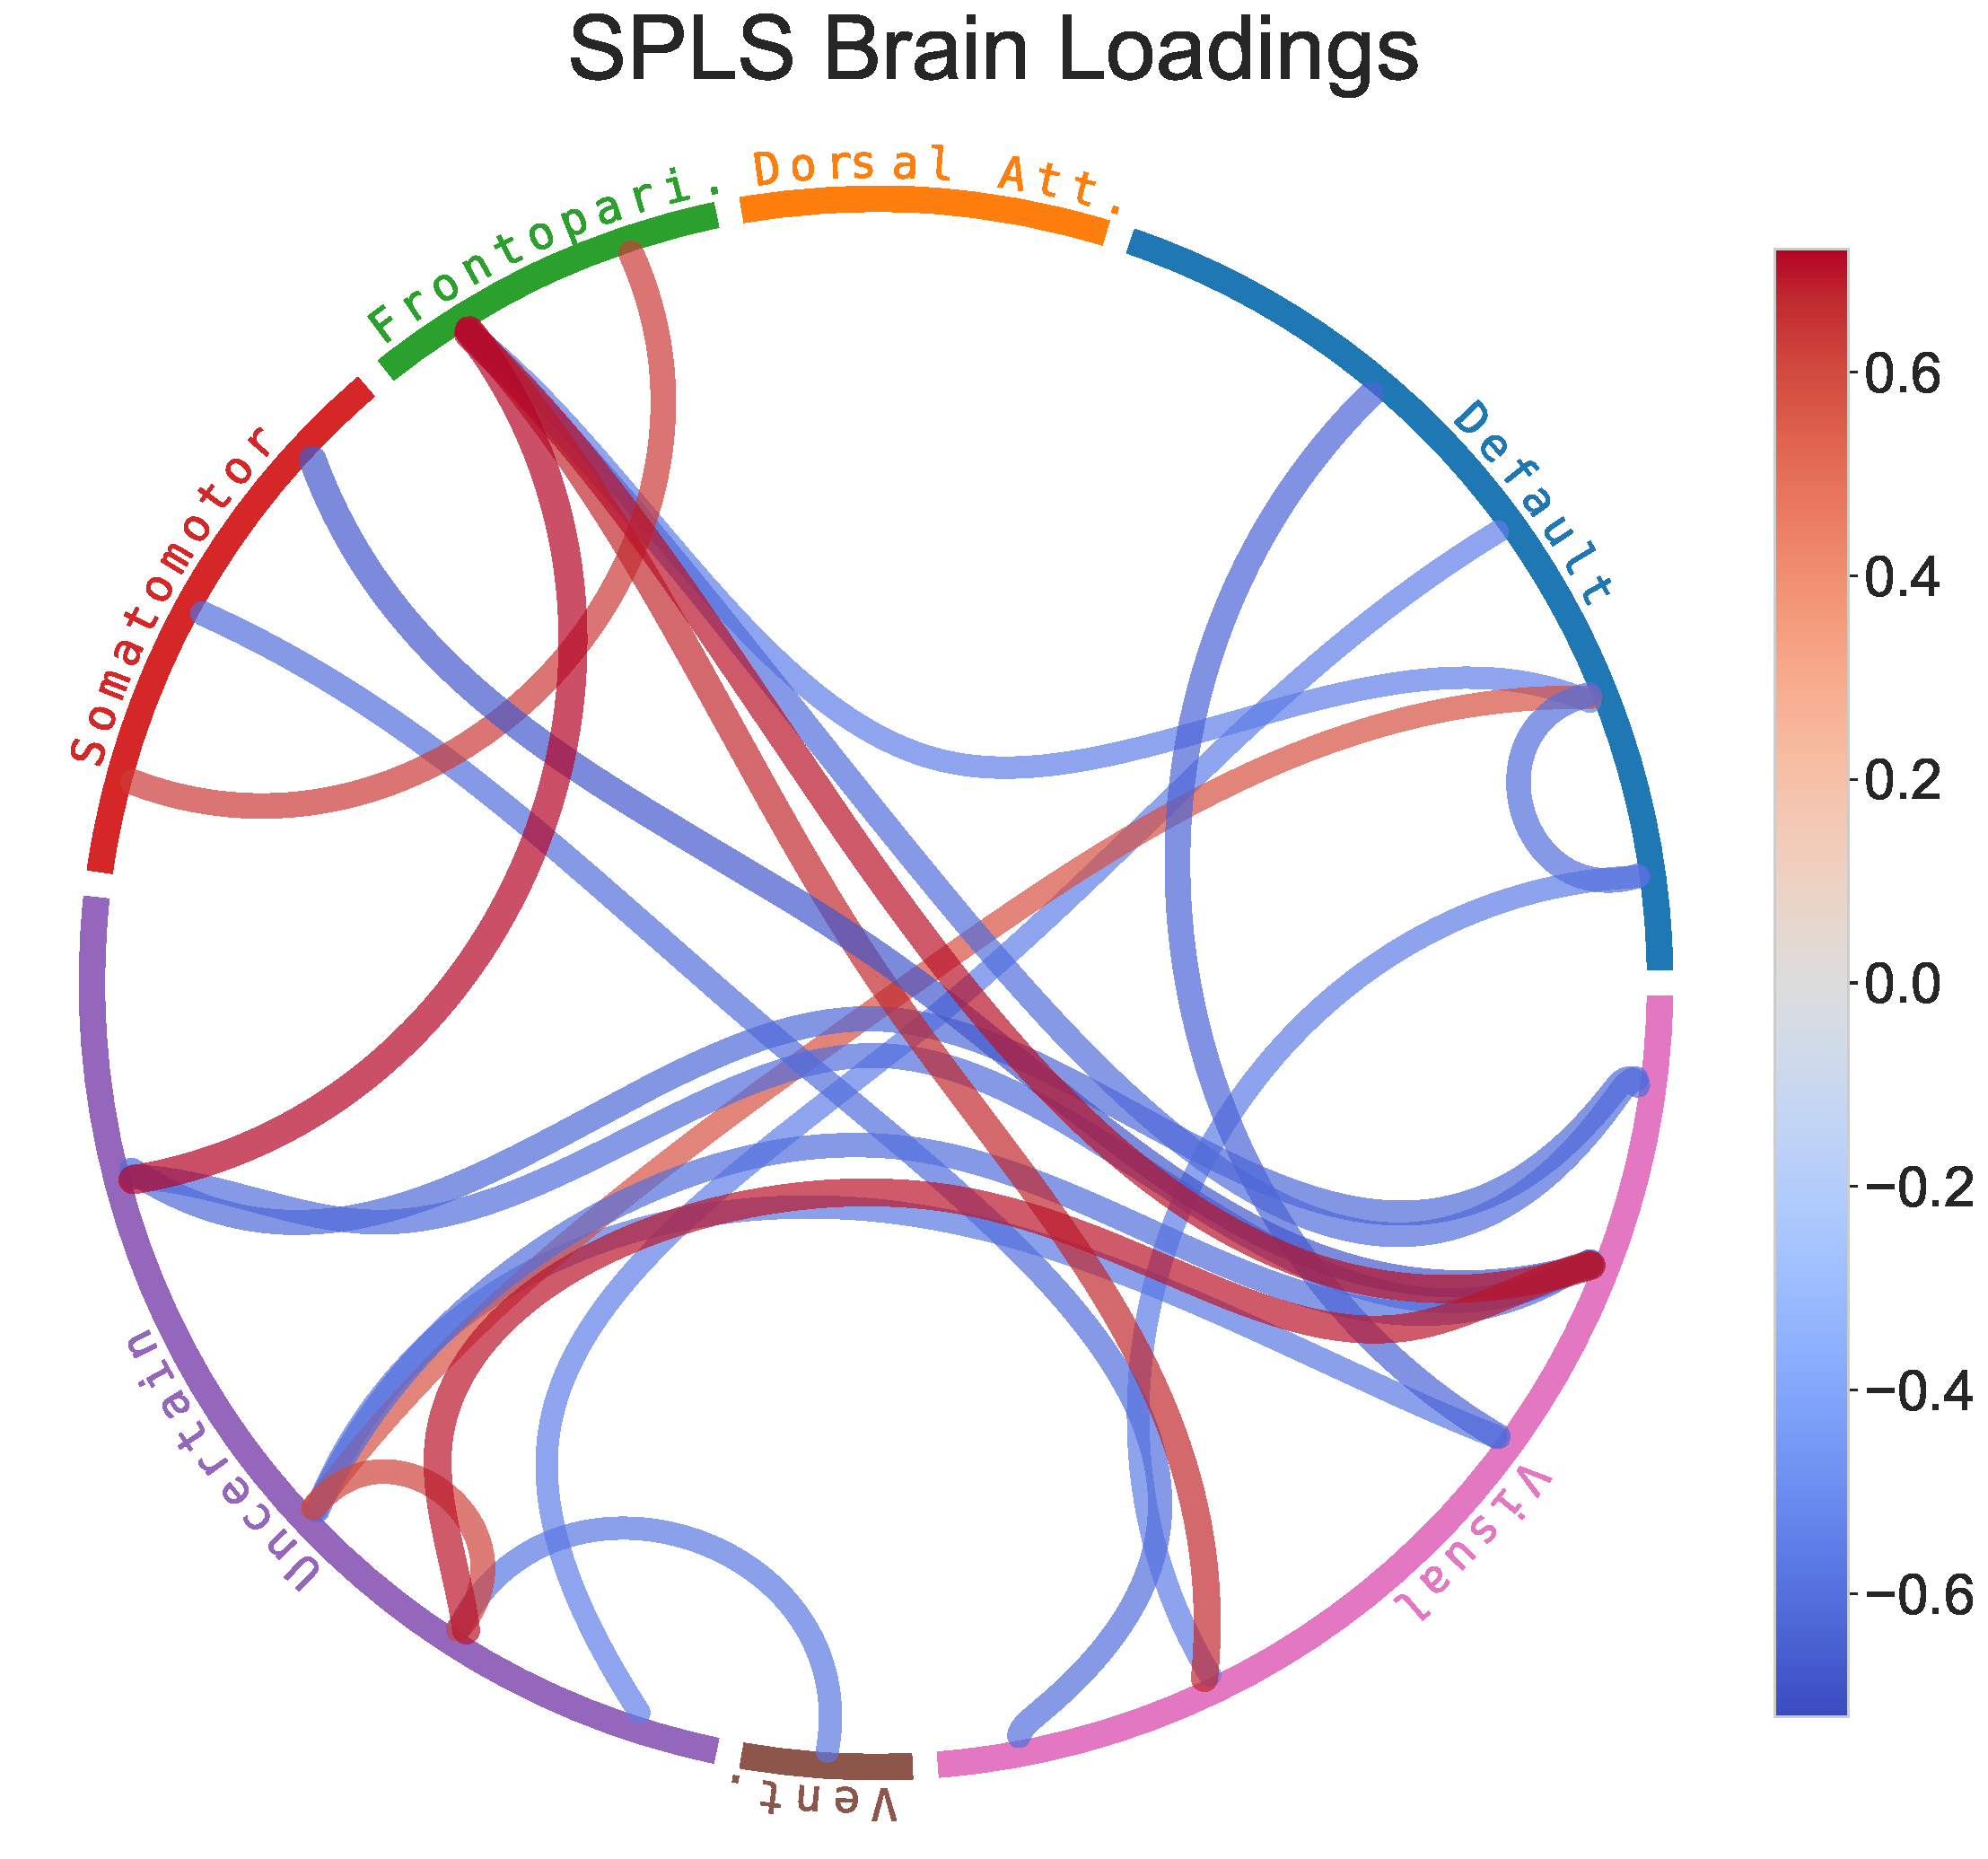
\includegraphics[width=0.49\linewidth]{figures/hcp/SPLS brain loadings}
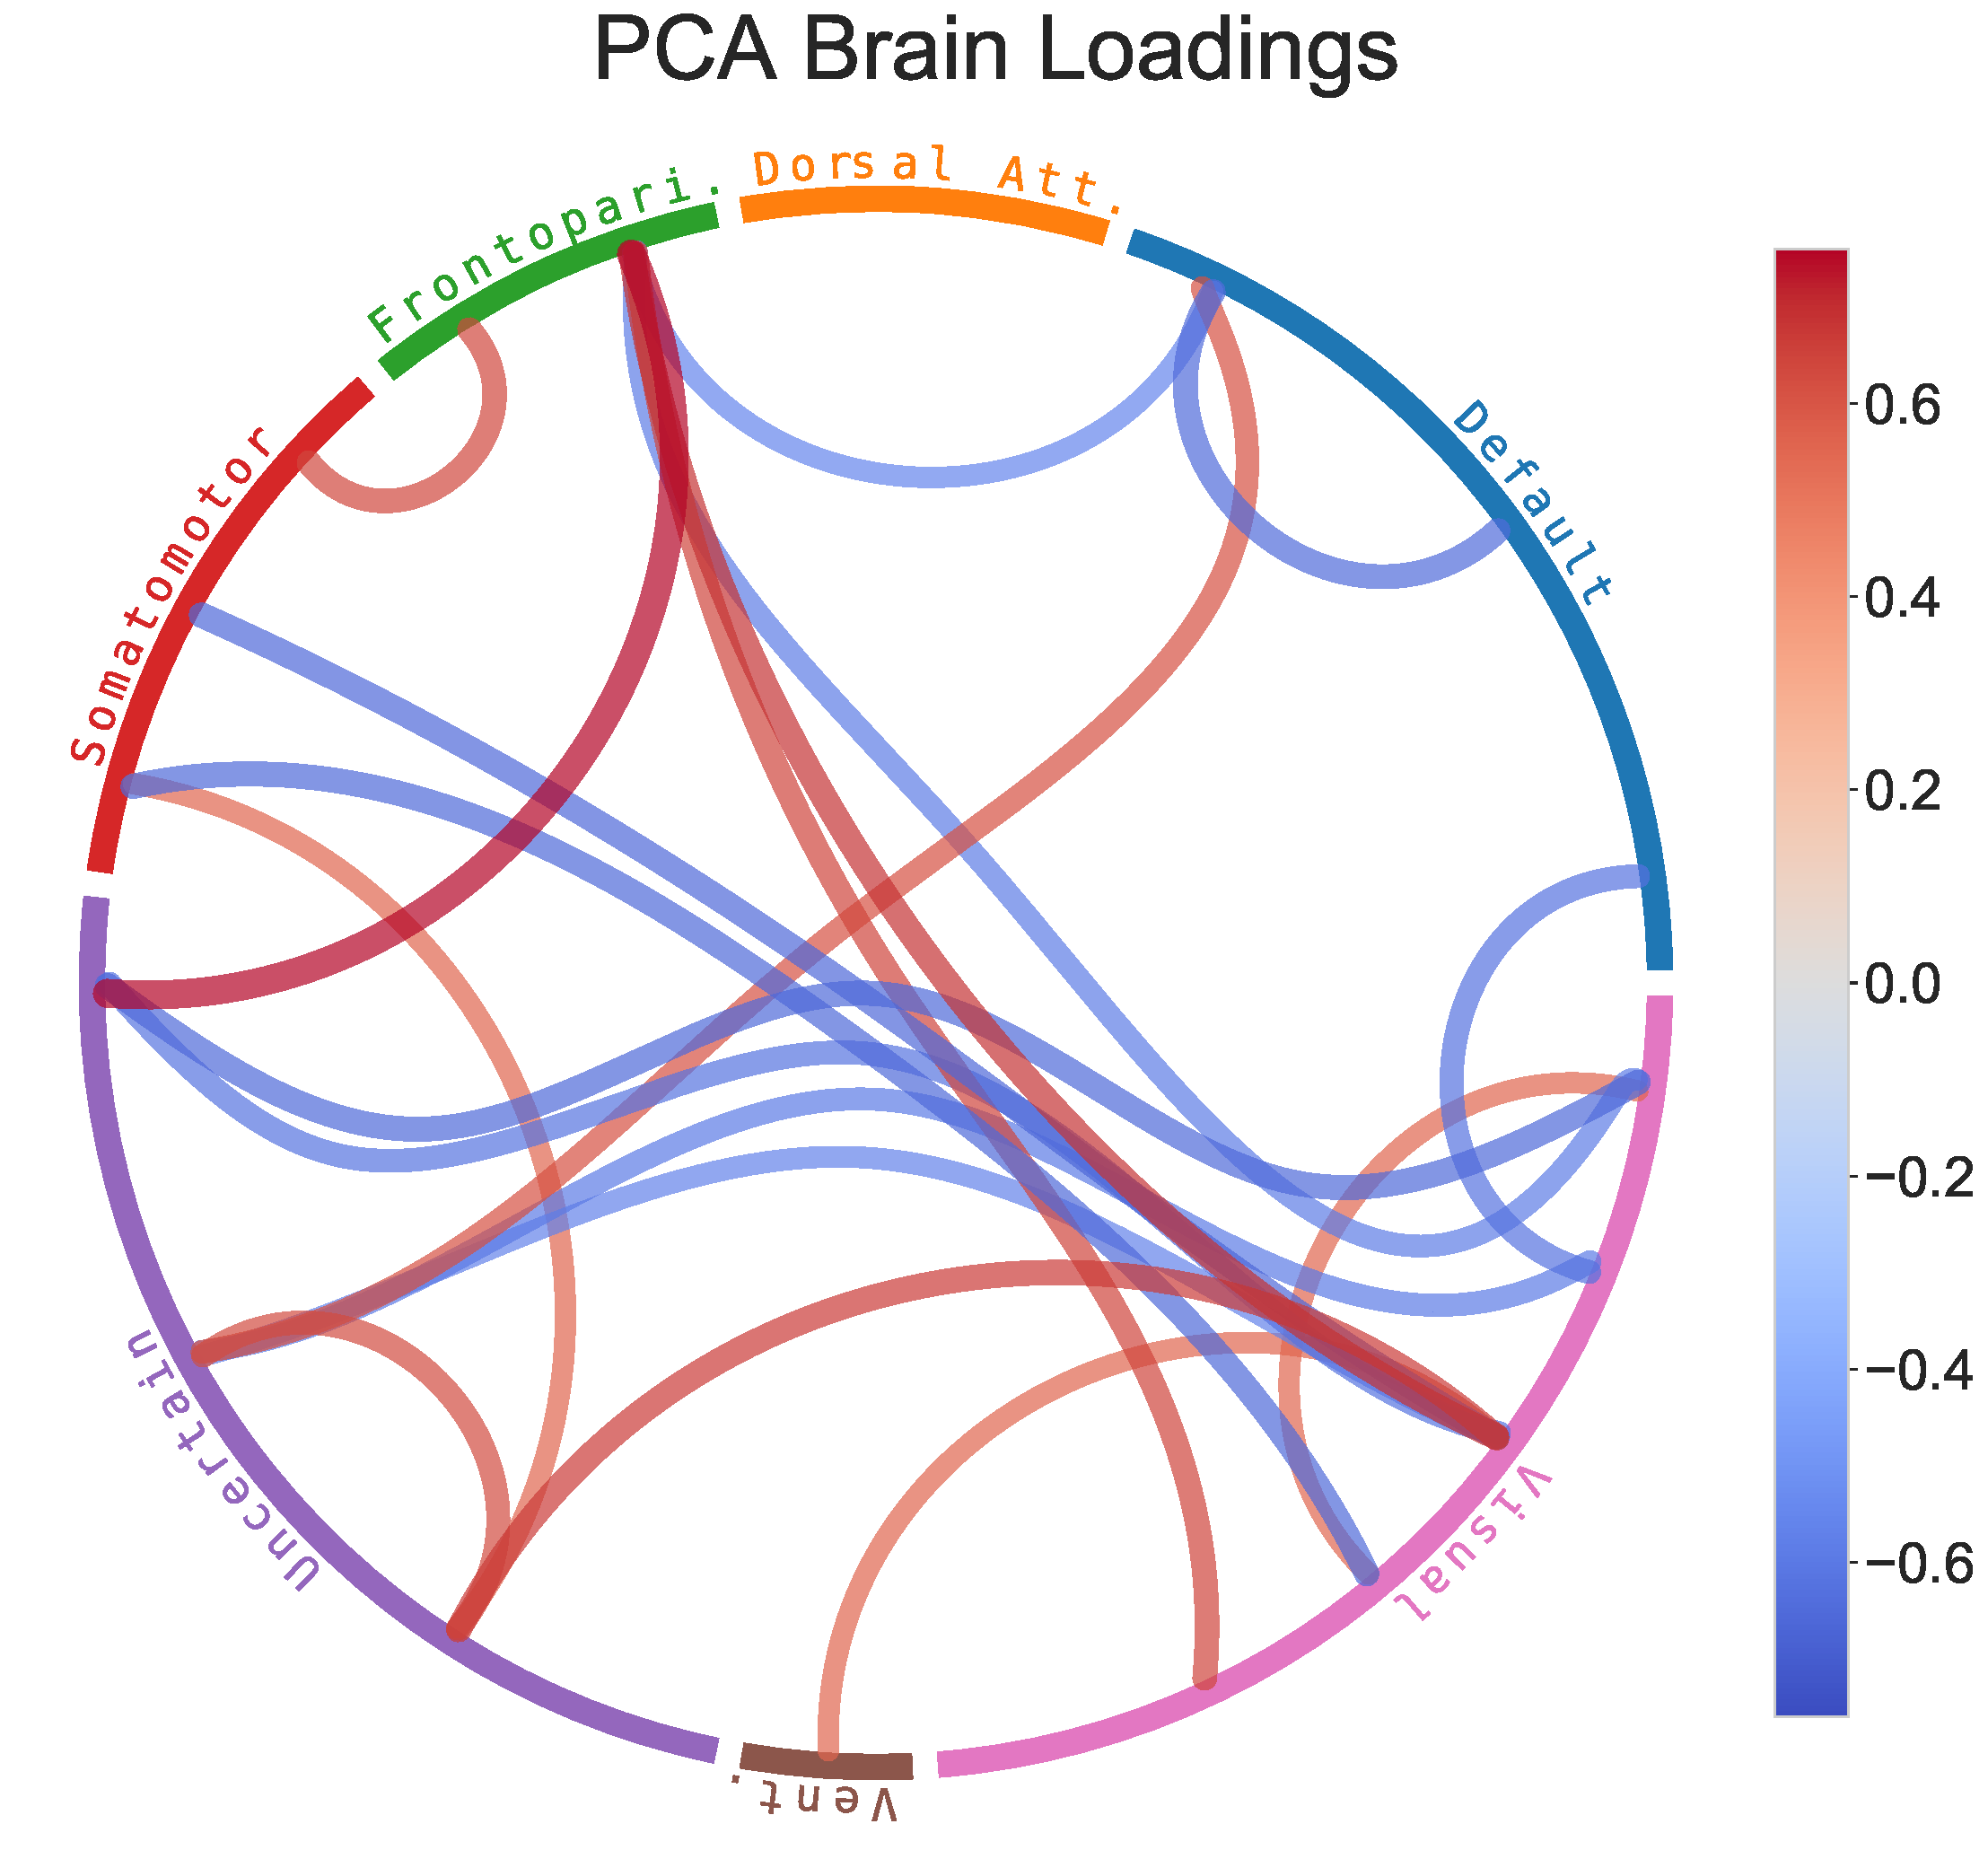
\includegraphics[width=0.49\linewidth]{figures/hcp/PCA brain loadings}
\caption{Chord diagrams of the top 8 positive and negative brain \gls{loadings} for each model.}\label{fig:chord_loadings}
\end{figure}

\newpage
\subsection{Alzheimer's Disease Neuroimaging Initiative (\acrshort{adni}) Data}

We now consider the \acrshort{adni} data.
Once again, we focus on the \gls{loadings} rather than the weights.

\subsubsection{Behaviour Weights and Loadings}



\begin{figure}
\centering
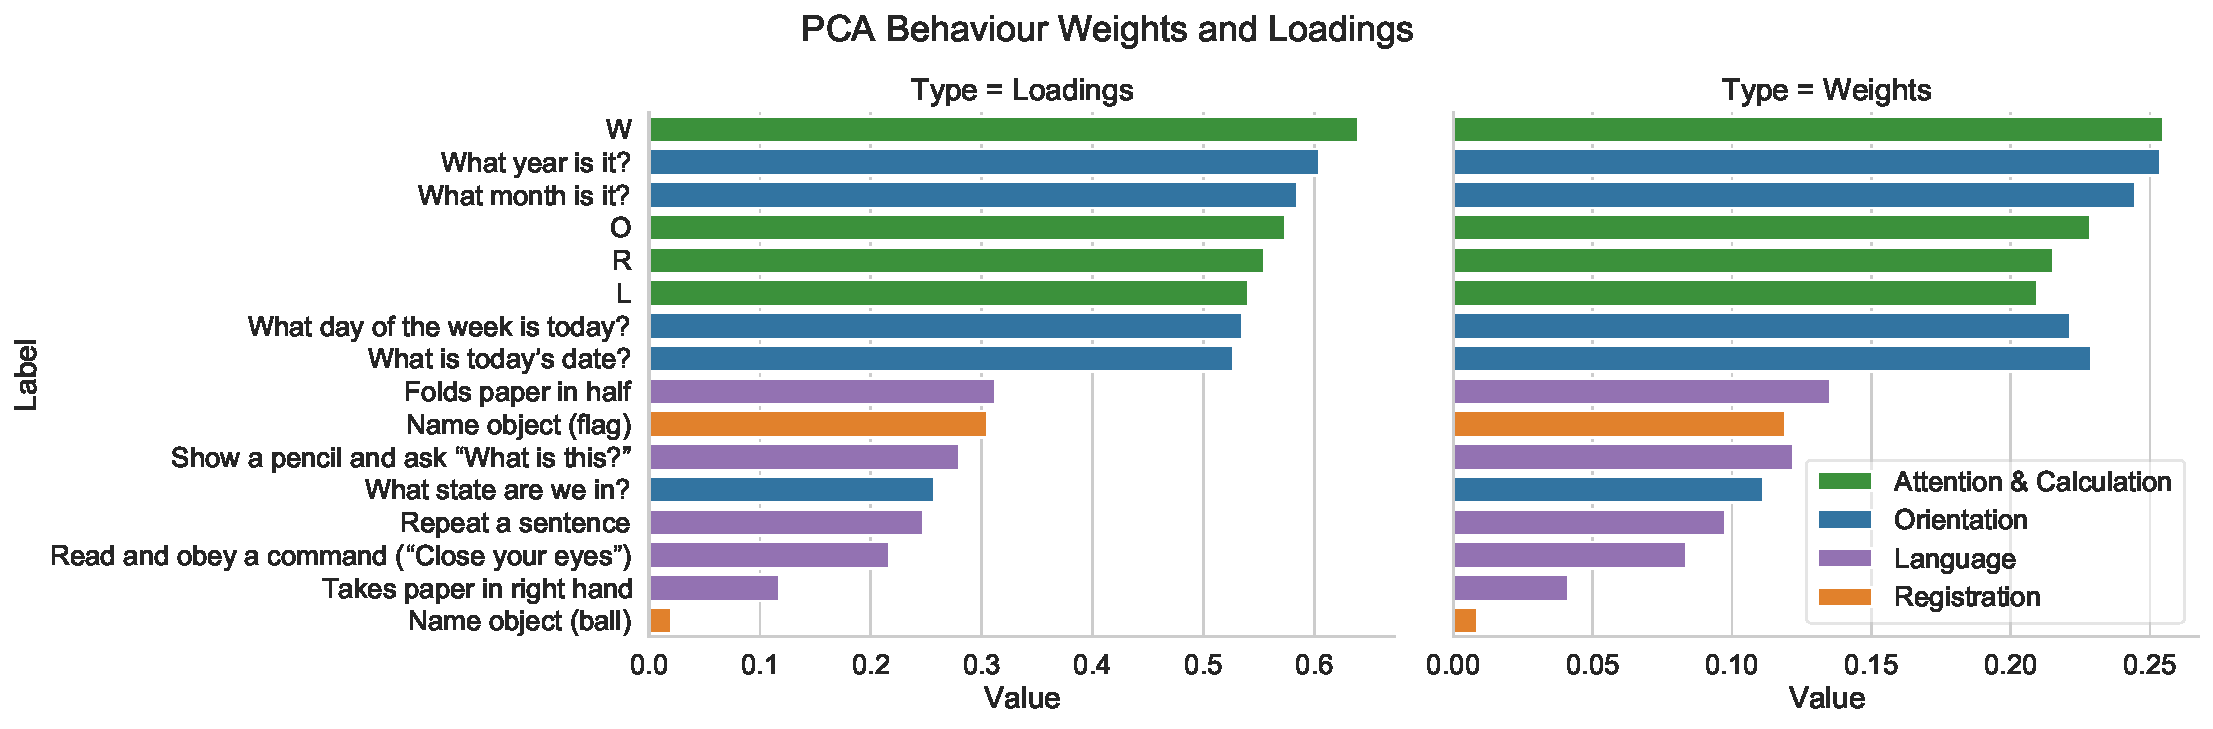
\includegraphics[width=0.8\linewidth]{figures/adni/PCA behaviour weights and loadings}
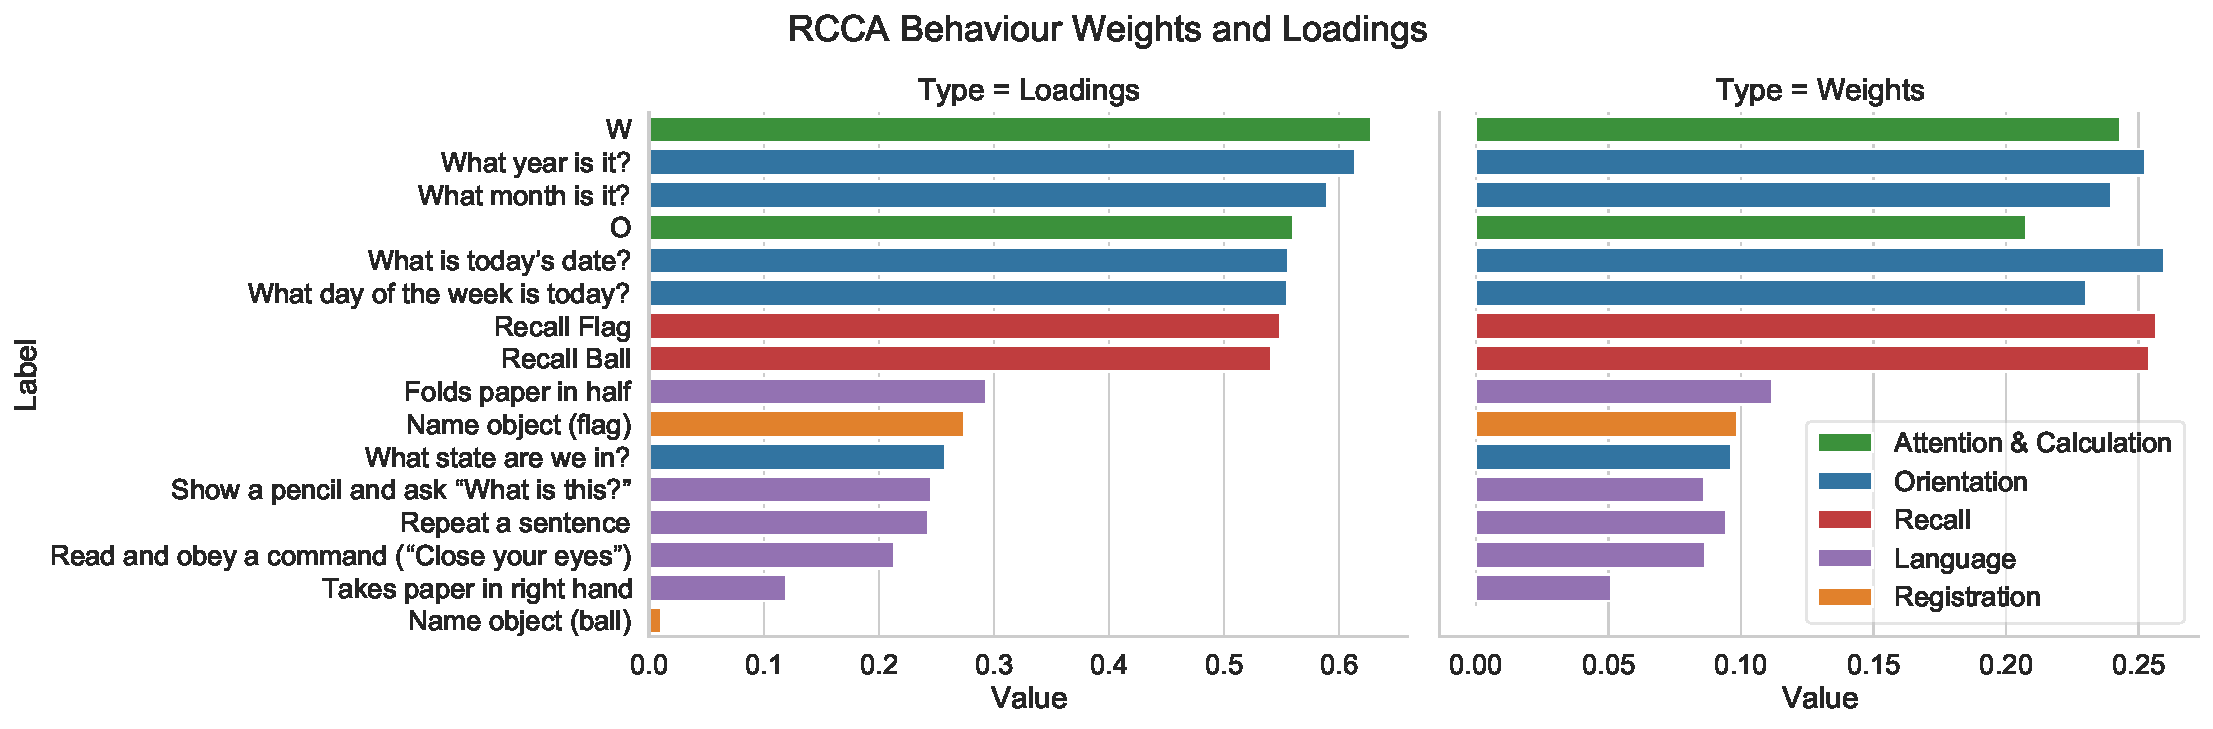
\includegraphics[width=0.8\linewidth]{figures/adni/RCCA behaviour weights and loadings}
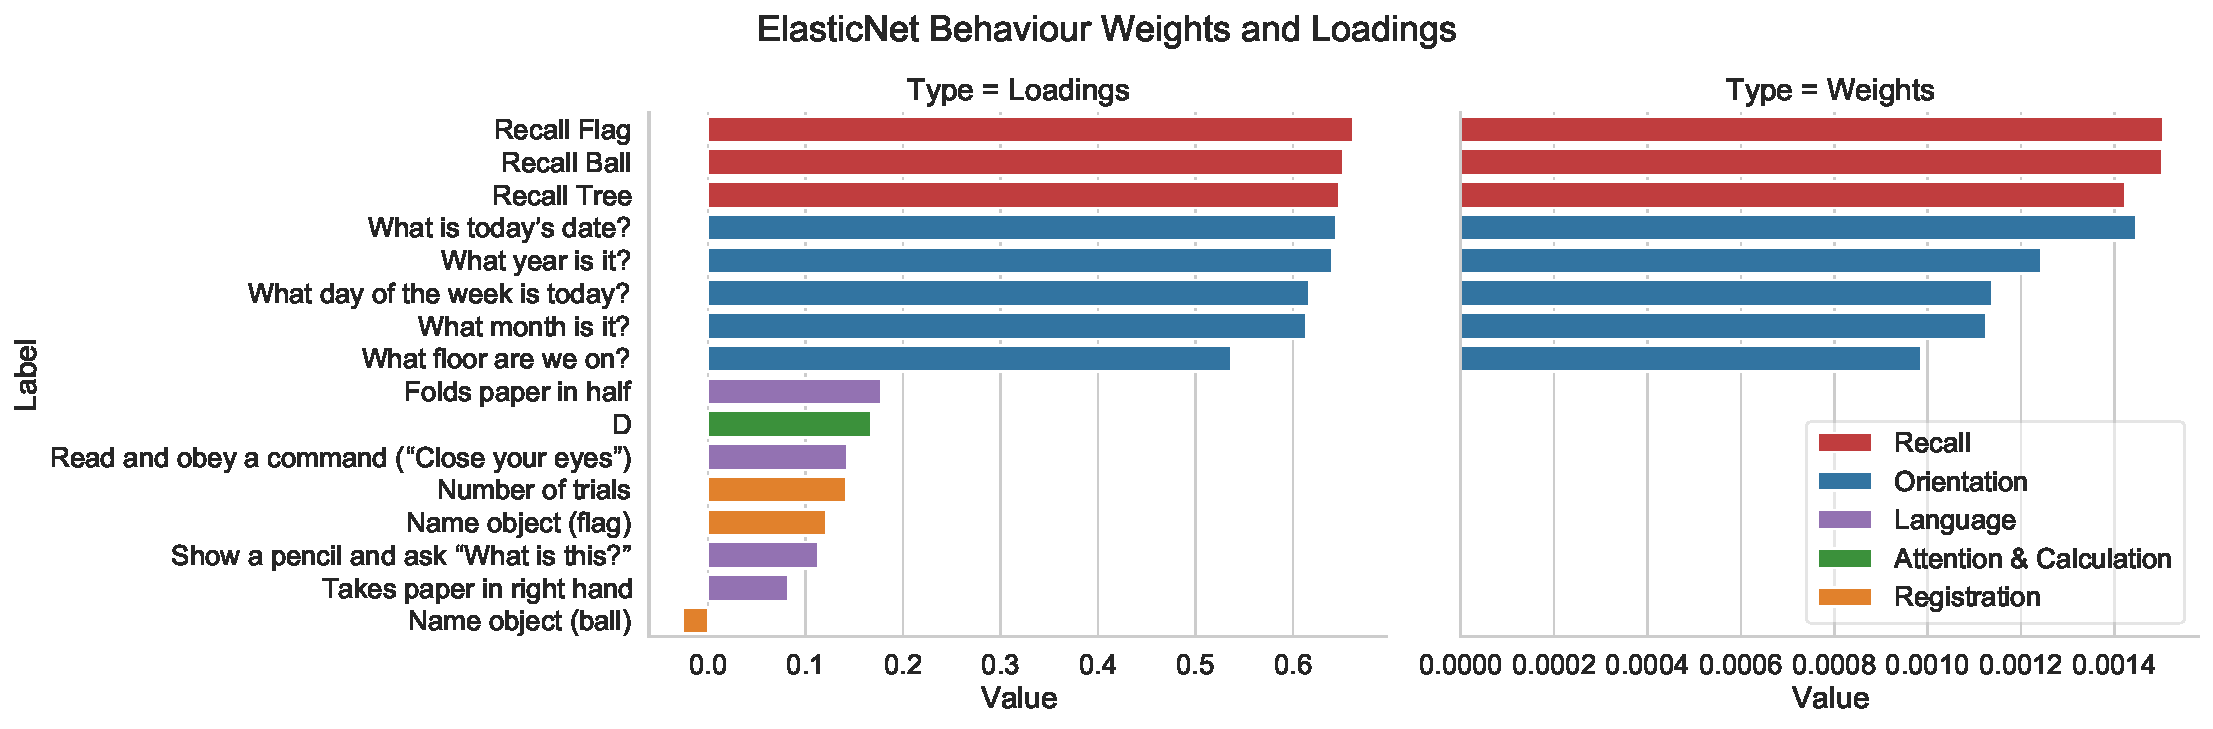
\includegraphics[width=0.8\linewidth]{figures/adni/ElasticNet behaviour weights and loadings}
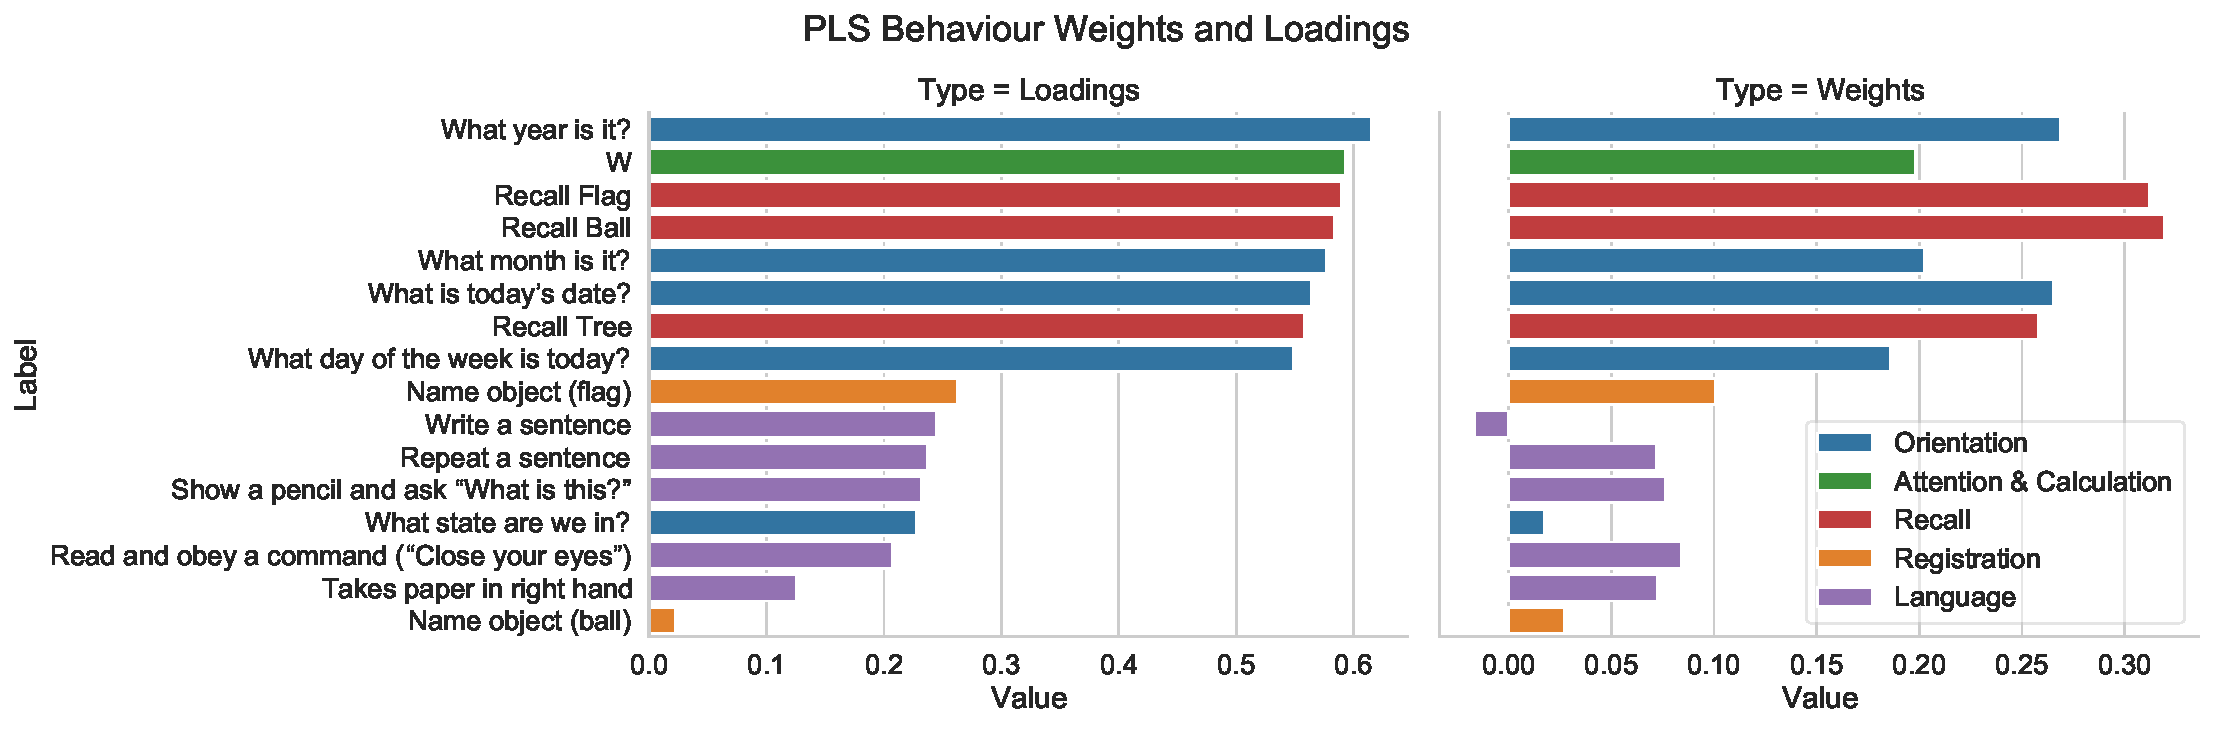
\includegraphics[width=0.8\linewidth]{figures/adni/PLS behaviour weights and loadings}
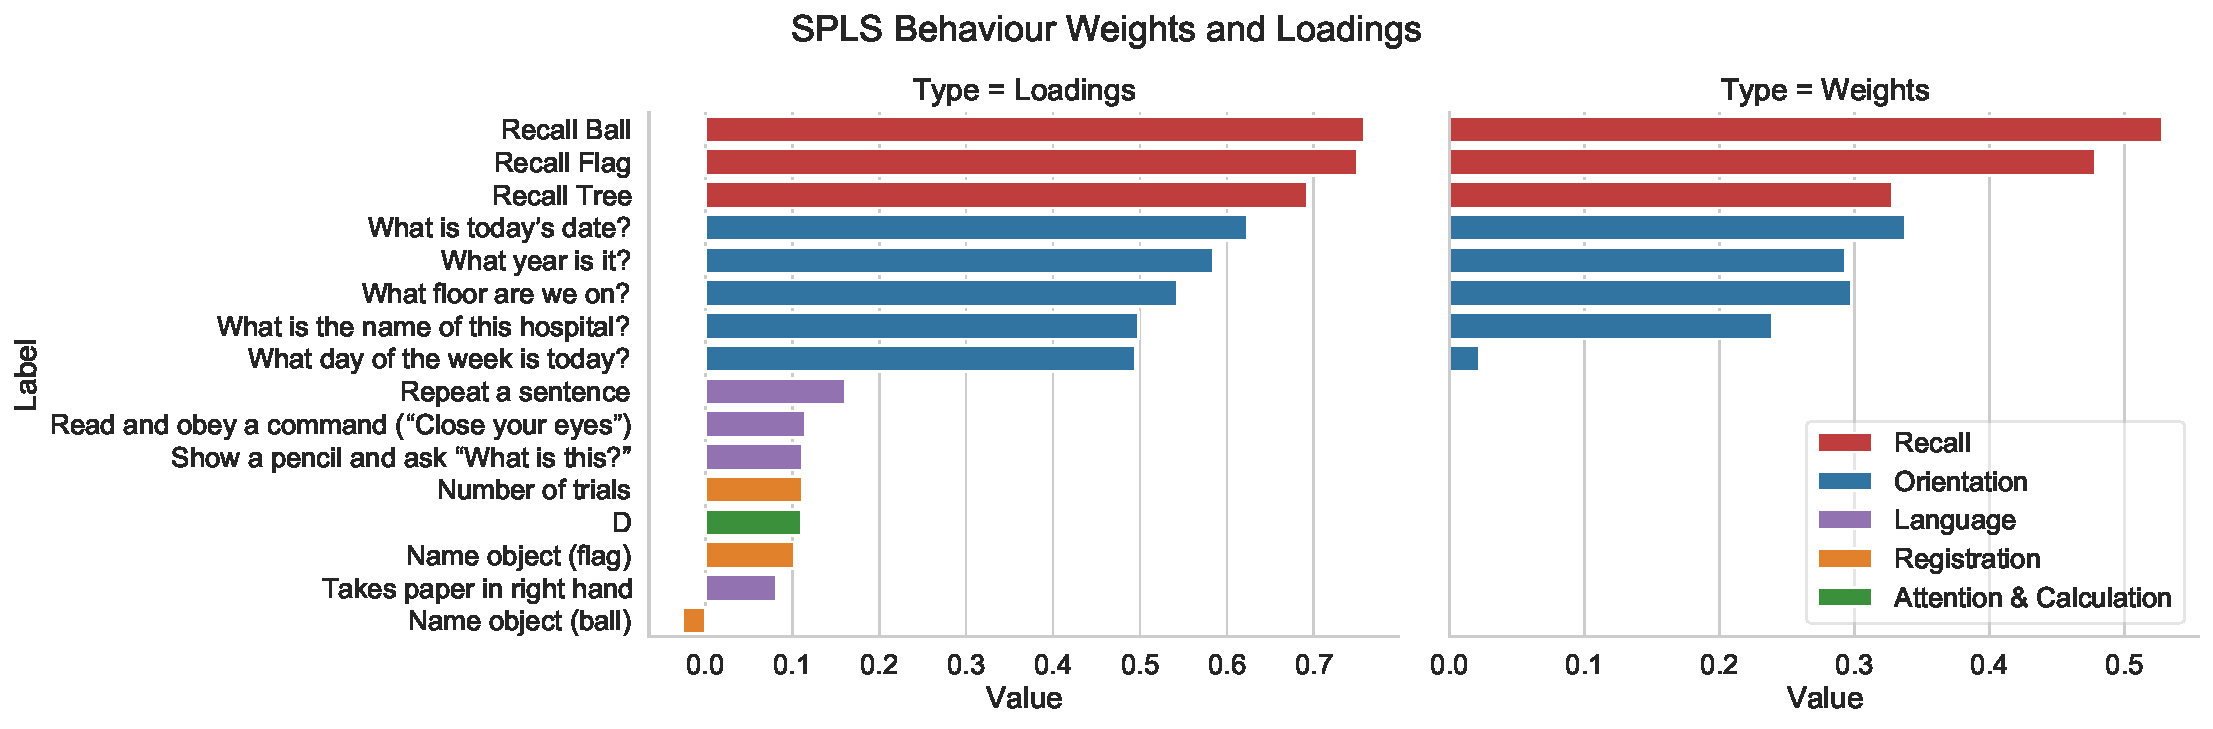
\includegraphics[width=0.8\linewidth]{figures/adni/SPLS behaviour weights and loadings}
\caption{Bar plots of the behaviour \gls{weights} and \gls{loadings} for each model.}
\end{figure}

\subsubsection{Brain Structure Weights and Loadings}

\begin{figure}
\centering
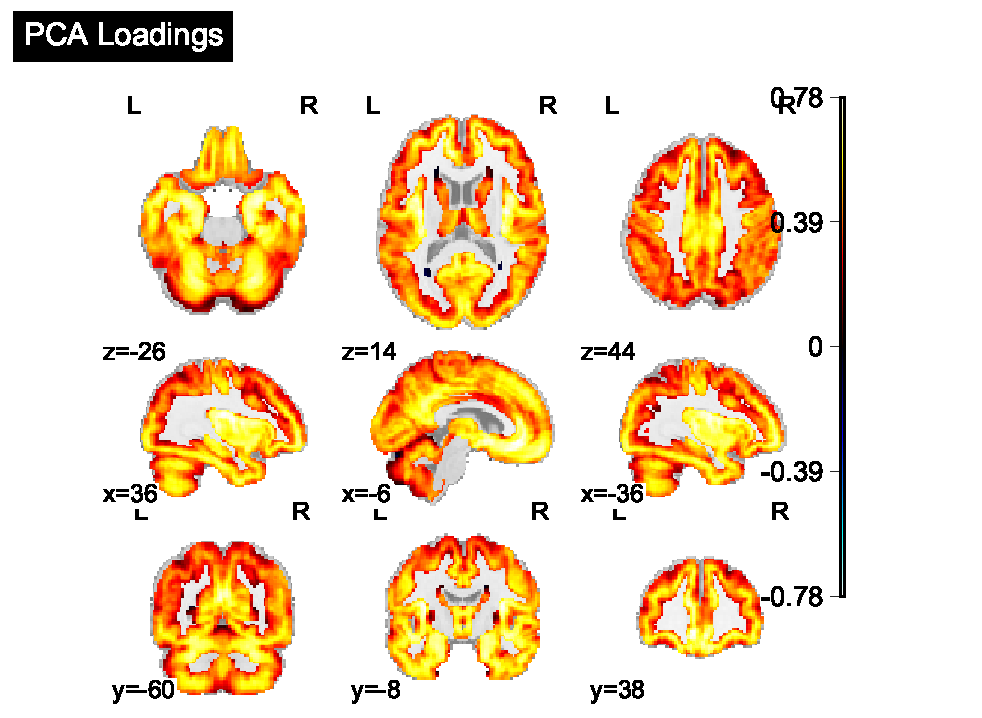
\includegraphics[width=0.45\linewidth]{figures/adni/PCA brain loadings mosaic}
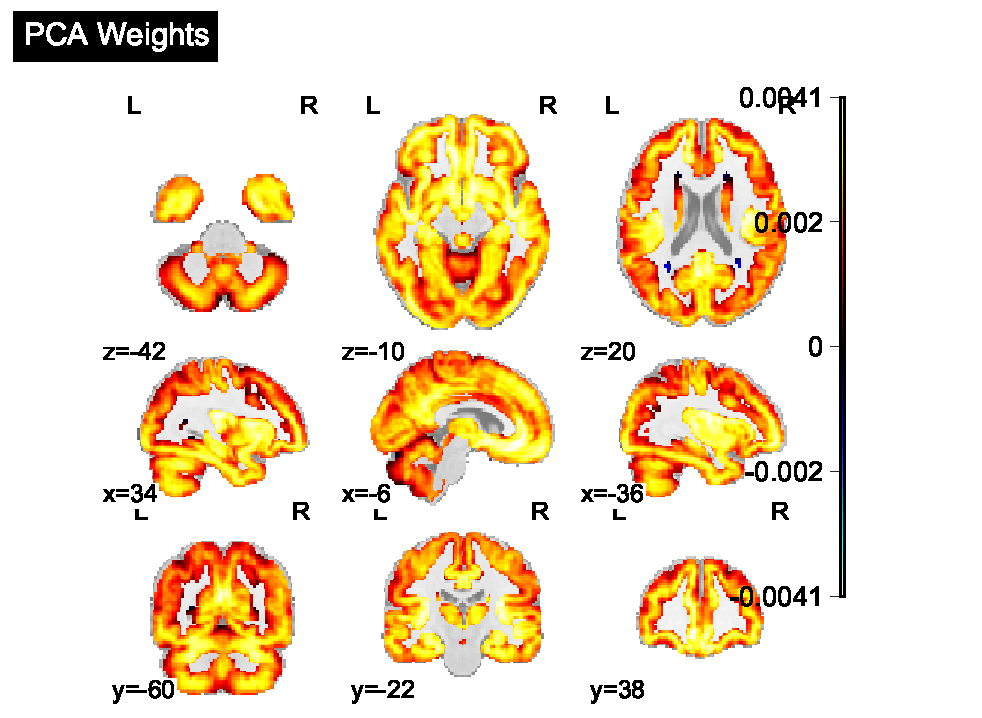
\includegraphics[width=0.45\linewidth]{figures/adni/PCA brain weights mosaic}
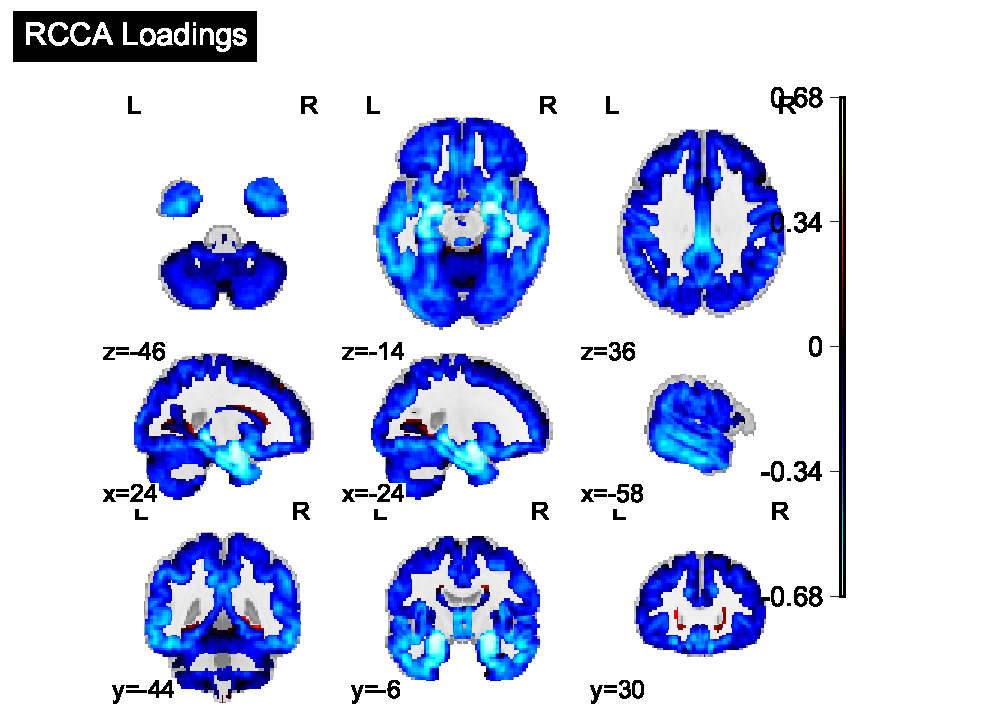
\includegraphics[width=0.45\linewidth]{figures/adni/RCCA brain loadings mosaic}
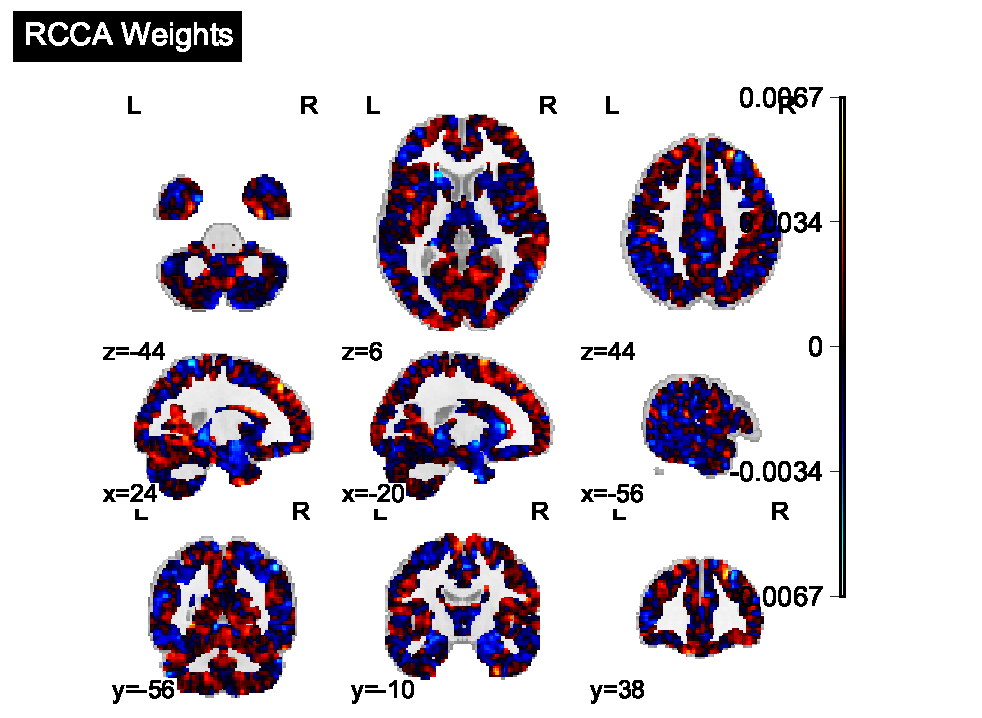
\includegraphics[width=0.45\linewidth]{figures/adni/RCCA brain weights mosaic}
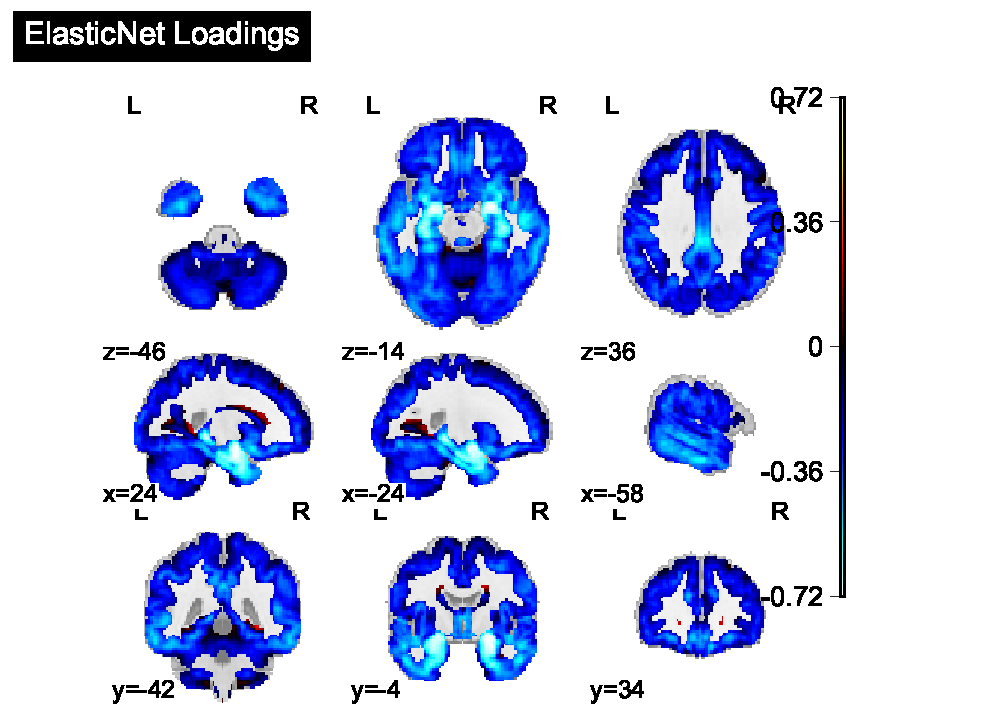
\includegraphics[width=0.45\linewidth]{figures/adni/ElasticNet brain loadings mosaic}
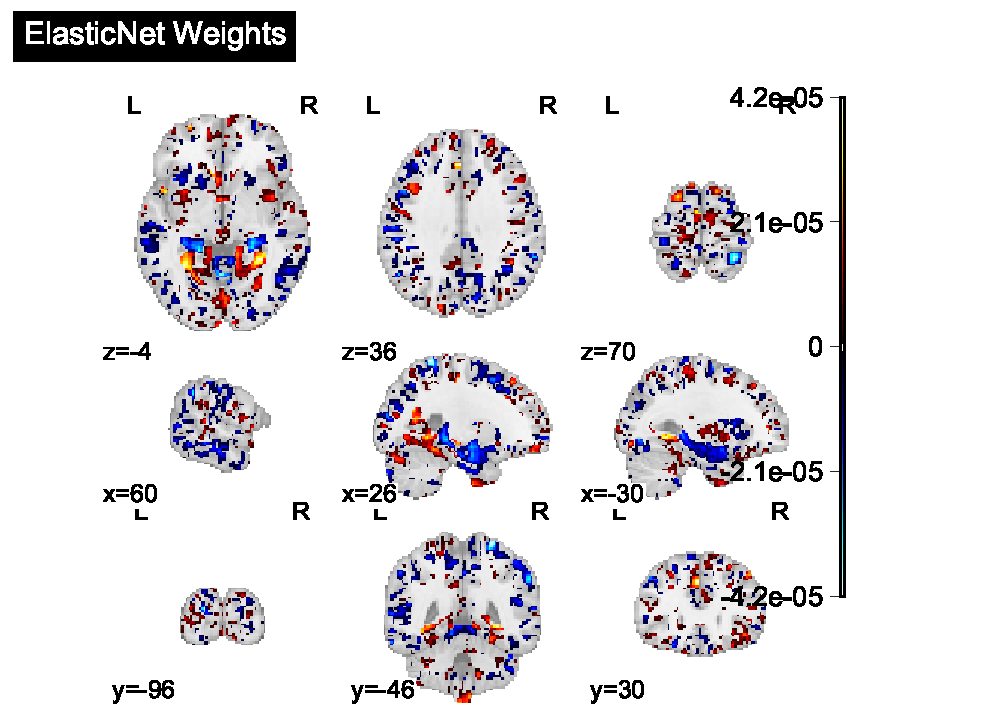
\includegraphics[width=0.45\linewidth]{figures/adni/ElasticNet brain weights mosaic}
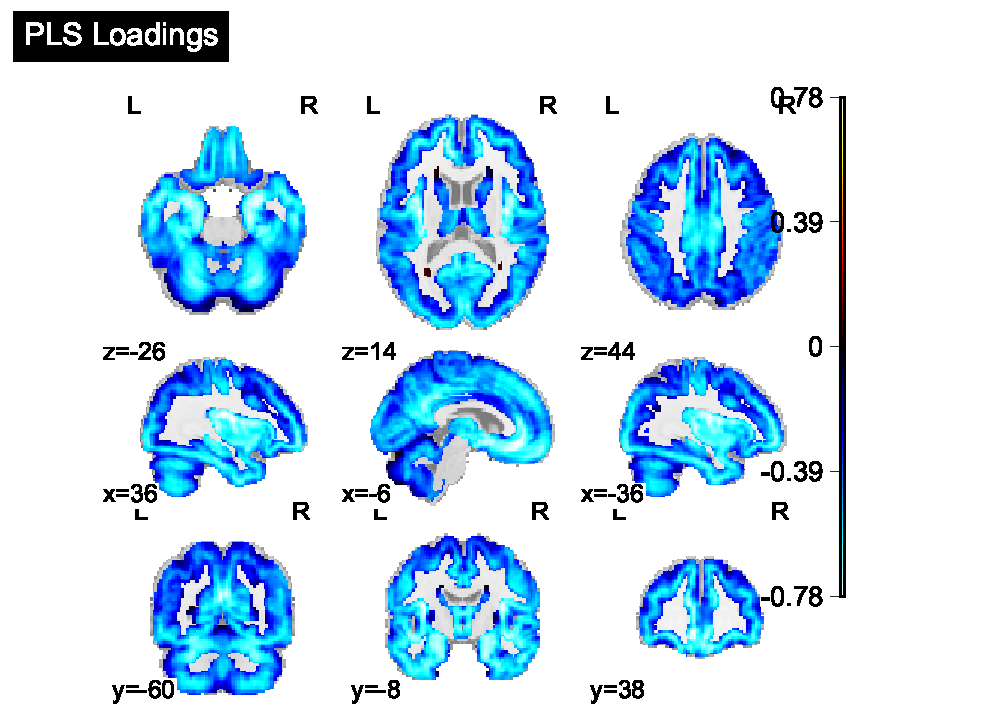
\includegraphics[width=0.45\linewidth]{figures/adni/PLS brain loadings mosaic}
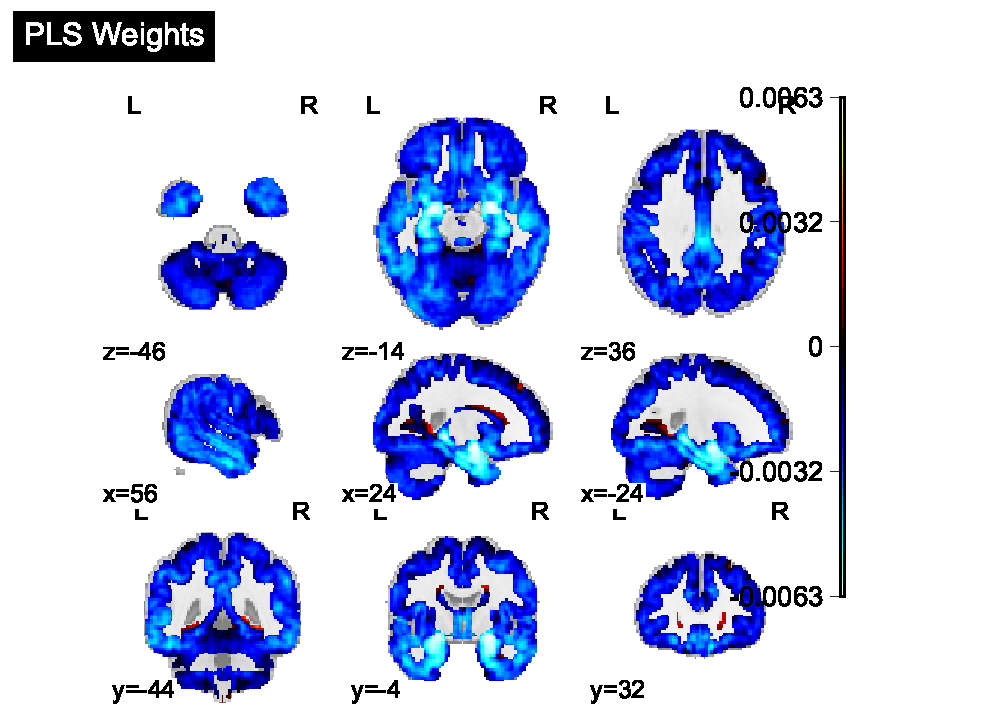
\includegraphics[width=0.45\linewidth]{figures/adni/PLS brain weights mosaic}
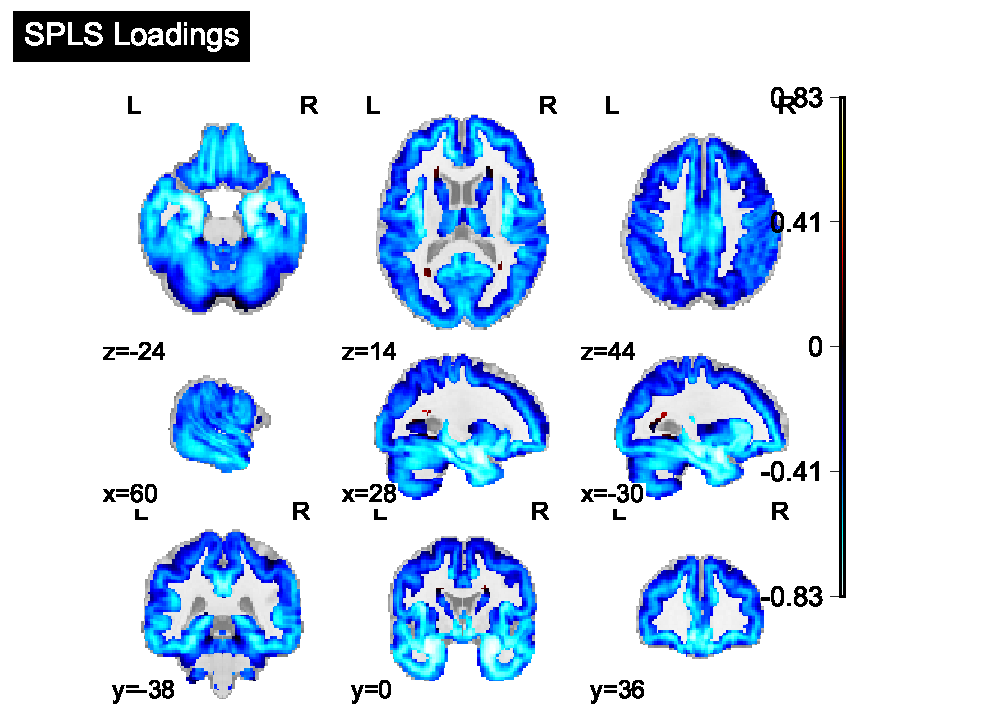
\includegraphics[width=0.45\linewidth]{figures/adni/SPLS brain loadings mosaic}
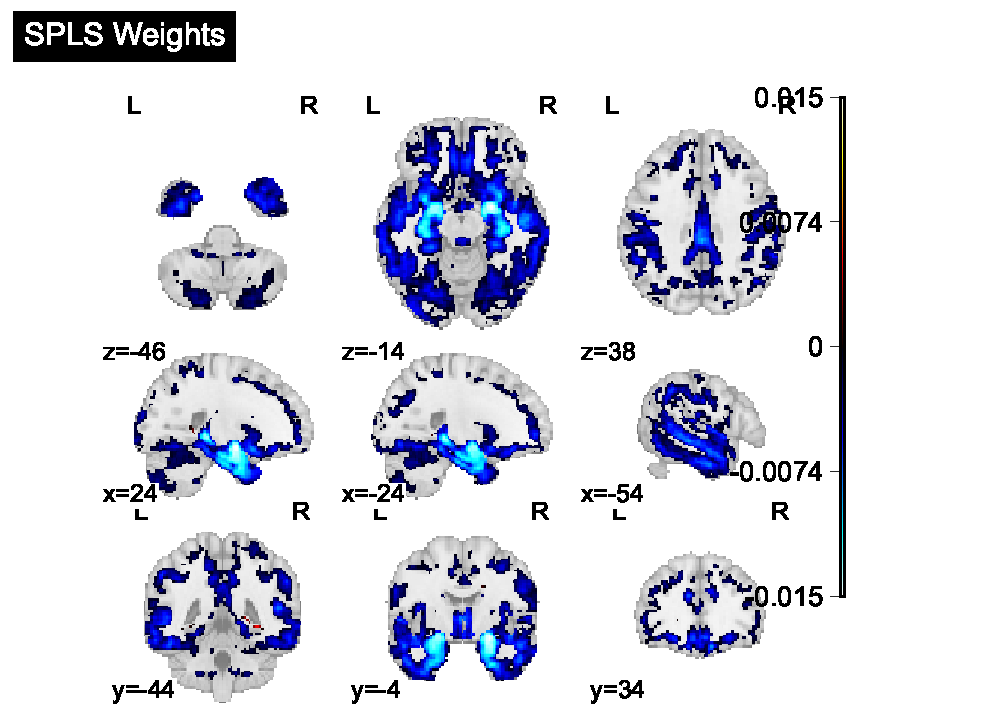
\includegraphics[width=0.45\linewidth]{figures/adni/SPLS brain weights mosaic}
\caption{Statistical maps of brain structure \gls{loadings} and \gls{weights} for each model.}\label{fig:adni-brain}
\end{figure}

\subsubsection{Identitiness of Covariance Matrices}
In this section, we consider the identitiness of the covariance matrices for the \acrshort{hcp} and \acrshort{adni} datasets.
Figure \ref{fig:covariance-eigenvalues-real} shows the eigenvalues of the covariance matrices for the \acrshort{hcp} and \acrshort{adni} datasets while Figure \ref{fig:covariance-matrices-real} shows the covariance matrices themselves (with the \acrshort{adni} brain covariance matrix left out due to its size).
From Figure \ref{fig:covariance-eigenvalues-real}, we can see that the eigenvalues of the covariance matrices for the \acrshort{adni} data are much closer to the ideal for identity covariance than for the \acrshort{hcp} data.
\begin{figure}
\centering
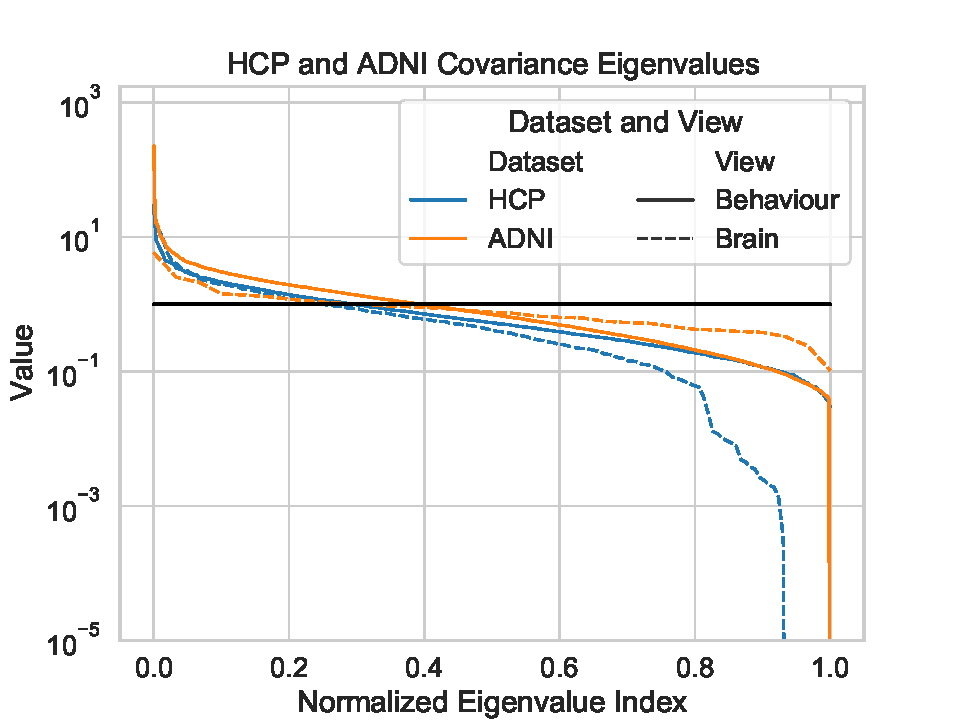
\includegraphics[width=0.8\linewidth]{figures/covariance/hcp_adni_covariance_eigenvalues}
\caption{Eigenvalues of the covariance matrices for the \acrshort{hcp} and \acrshort{adni} datasets.}\label{fig:covariance-eigenvalues-real}
\end{figure}

From Figure \ref{fig:covariance-matrices-real}, we can see the block structure of the covariance matrices.

\begin{figure}
\centering
\begin{subfigure}{0.66\linewidth}
\centering
\includegraphics[width=\linewidth]{figures/covariance/hcp_covariance}
\caption{\acrshort{hcp}}
\end{subfigure}
%
\begin{subfigure}{0.33\linewidth}
\centering
\includegraphics[width=\linewidth]{figures/covariance/adni_covariance}
\caption{\acrshort{adni}}
\end{subfigure}
\caption{Covariance matrices for the \acrshort{hcp} and \acrshort{adni} datasets.}
\label{fig:covariance-matrices-real}
\end{figure}

\section{Discussion and Limitations}

In this section, we discuss the implications of our findings as well as the limitations of our study.

\subsection{Discussion}

\paragraph{Interpreting the Forward and Backward Models of \acrshort{cca}:} Consistent with \cite{haufe2014interpretation}, we have shown that assumptions imposed on the \gls{weights} of a model do not in general transfer to the loadings.
This is because the \gls{weights} and \gls{loadings} are only equivalent when the covariance matrices are identity.
We have gone a step further than \cite{haufe2014interpretation} by showing that the identitiness of the covariance matrices is crucial for understanding how imposing sparsity on the \gls{weights} imposes a prior belief in sparsity on the more biologically interesting loadings.

\paragraph{Sparsity on the \gls{weights} does not imply sparsity on the loadings:}

On the other hand, our results raise whether sparsity on the \gls{weights} makes sense in the first place.
For latent variable models of brain-behaviour associations, we have argued that the \gls{loadings} are the more biologically relevant quantity.
Since in practice, identity covariance is rarely a good assumption, the \gls{weights} and \gls{loadings} are not equivalent.
This means that sparsity on the \gls{weights} does not imply sparsity on the loadings, and so we should not expect sparsity on the \gls{weights} to lead to more interpretable loadings.
A practical step this implies is \textit{to ensure that the data covariances are at least close to identity before applying sparse \acrshort{cca} methods}.

\paragraph{Identitiness of real covariance matrices:} Between the \acrshort{hcp} and \acrshort{adni} datasets, only the \acrshort{adni} data had eigenvalue spectra that were reasonably close to those of an identity matrix.
This suggests that the only dataset and view where we can expect sparsity on the \gls{weights} to imply sparsity on the \gls{loadings} is the \acrshort{adni} data.
This is consistent with the results we have seen in the previous section, that sparsity improves performance in the \acrshort{adni} data but not in the \acrshort{hcp} data.
Furthermore, the \gls{loadings} and \gls{weights} are much more similar to each other in the \acrshort{adni} data than in the \acrshort{hcp} data, supporting the idea that the \acrshort{adni} \gls{weights} are themselves somewhat interpretable as estimates of the biologically relevant loadings.
Finally, in the well understood Alzheimer's disease data, we know that the identified \gls{weights} (and loadings) are consistent with the known biology of the disease.

\paragraph{Sample versus Population Setting:} The results from the simulated data illustrate the disparities that can arise between population and sample settings.
Although \acrshort{pls}, \acrshort{rcca}, and \acrshort{cca} are equivalent under isotropic noise in a population framework, experiments showed that their performance can vary substantially in a sample setting.
In particular, this manifested as \acrshort{pls} underperforming \acrshort{rcca} and \acrshort{cca} under isotropic noise \textit{even though this is exactly the scenario where covariance identity holds and covariance thus equals correlation}.
This is because the sample covariance matrix is not the same as the population covariance matrix and \acrshort{pls} is sensitive to even small differences in the principal components of the sample covariance matrix.
Furthermore, in limited sample sizes, our estimations of the covariance matrices are not accurate, and so the identitiness of the covariance matrices is not guaranteed.
This generally resulted in poor estimation of \gls{loadings} from model \gls{weights} \textit{even when the \gls{weights} themselves were estimated almost perfectly}.
Therefore, it's crucial for researchers to recognize these nuances and adopt appropriate measures when extrapolating results, especially in brain-behavior studies where typically only one sample is available and often limited in size.

\paragraph{Ridge \acrshort{cca} is typically much better than \acrshort{pls} across datasets:} Our results show that Ridge \acrshort{cca} is typically much better than \acrshort{pls} across datasets.
Much like regularised regression, it is unusual to need to use maximal ridge regularization even in high dimensions.
Our results in simulated data even cast doubt on the touted stability of \acrshort{pls} over \acrshort{cca} with respect to population \acrshort{cca} problem.
This means that while \acrshort{pls} might be more stable for a given dataset, it is not necessarily more stable across random samples from the same population.

\paragraph{Can We Construct a Regularization Functional that Imposes Sparsity on the Loadings?}
Finally, given our observations, a natural question to ask is whether we can construct a regularization functional that imposes sparsity on the \gls{loadings} (instead of the weights).
The answer is yes, but it is not straightforward and in the small sample setting, it is not clear that it is a good idea.
The principle would be much the same as the Lasso, but we would need to use the sample covariance matrix to define the norm:

\begin{align}
    P(W)=\|W\|_1 \\
    P(L)=\|\hat{\Sigma}U\|_1
\end{align}

Which imposes an L1 penalty on the \gls{loadings} via an L1 penalty on the \gls{weights} multiplied by the sample covariance matrix.
We could in principle apply the soft-thresholding operator to the estimated loadings.
However we would need to be careful to ensure that the sample covariance matrix is invertible in order to get back to the weights.
This is of course not guaranteed in the small sample setting.

\section{Conclusion}

In this chapter, we have explored the performance of several \acrshort{cca} variants on simulated and real data.
We have shown that the choice of \acrshort{cca} variant can have a significant impact on the results.
We have also shown that the identitiness of the covariance matrices is crucial for understanding how imposing sparsity on the \gls{weights} imposes a prior belief in sparsity on the more biologically interesting loadings.
We described a way to check the identitiness of the covariance matrices by looking at the eigenvalues of the covariance matrices and comparing to the ideal case.
In the next chapter, we address the scalability of \acrshort{cca} and its variants by introducing a novel algorithm based on gradient descent.